\documentclass[times, utf8, diplomski]{fer}
\usepackage{booktabs}
\usepackage{listings}
\usepackage{afterpage}
\usepackage{color}
\usepackage{caption}
\usepackage{float}
\usepackage{pdfpages}
\usepackage{backnaur}
\usepackage[croatian, croatiankw, onelanguage, vlined, boxruled]{algorithm2e}
\usepackage[]{graphicx}
\usepackage{subfig}
\usepackage[export]{adjustbox}
\usepackage{array}
\usepackage{multirow}

\renewcommand{\algorithmcfname}{Pseudokod}
\newcounter{nalg}[chapter]
\renewcommand{\thenalg}{\thechapter .\arabic{nalg}}

\begin{document}

% TODO: Navedite broj rada.
\thesisnumber{2020}

% TODO: Navedite naslov rada.
\title{Izvedba vektorskih Booleovih funkcija temeljena na konfigurabilnim logičkim blokovima}

% TODO: Navedite svoje ime i prezime.
\author{Luka Suman}

\maketitle


\includepdf{img/izvornik.pdf}

% Dodavanje zahvale ili prazne stranice. Ako ne želite dodati zahvalu, naredbu ostavite radi prazne stranice.
\zahvala{}

\tableofcontents

\chapter{Uvod} \label{chapter:introduction}

%TODO

\chapter{Opis problema} \label{chapter:problem}

Ovo poglavlje sadrži teoriju potrebnu za razumijevanje problema koji se razmatra u ostatku ovog rada. Odjeljak \ref{sec:bool-func} objašnjava Booleove funkcije. Prvo se definira pojam Booleove funkcije. Zatim slijedi kratko objašnjenje binarnog prikaza brojeva. Potom slijede $3$ načina prikaza Booleove funkcije: tablica istinitosti, kanonski oblik te Booleov izraz. Odjeljak \ref{sec:fpga} objašnjava FPGA uređaje. Navedene su osnove digitalnih sklopova koji se koriste u FPGA tehnologiji uz kratak pregled osnovnih svojstava. Na kraju je dana definicija problema u odjeljku \ref{sec:decomposition}.

%%%%%
%%%%%
%%%%%

\section{Booleove funkcije} \label{sec:bool-func}

Booleova funkcija je matematička funkcija definirana unutar grane matematičke algebre koja se zove Booleova algebra. Nju je uveo američki matematičar, filozof i logičar George Boole 1847.~godine. Naziv Booleova algebra predložen je 1913.~godine te se smatra da je Booleova algebra poslužila kao temelje za današnje informacijsko doba. Booleova funkcija je oblika $f:\boldsymbol{B}^{k}\mapsto \boldsymbol{B}$ gdje je $\boldsymbol{B}=\{0, 1\}$ Booleova domena, a $k$ je broj ulaznih varijabli. Prva vrijednost Booleove domene predstavlja logičku neistinu, dok druga vrijednost predstavlja logičku istinu. Postoji više načina označavanja tih dviju vrijednosti. U propozicijskoj logici često se koriste $\{\bot, \top \}$ i $\{F, T\}$ (engl.~\textit{$\{False, True\}$}), dok se u digitalnoj logici najčešće koriste $\{0, 1\}$. Razlika između Booleove algebre i matematičke algebre jest u predmetu proučavanja. Booleova algebra proučava binarne vrijednosti ($0$ i $1$) umjesto brojeva (cijeli, racionalni, itd.) te proučava logičke operacije umjesto matematičkih operacija (zbrajanje, množenje, itd). Booleove funkcije imaju široku primjenu u teoriji računarstva, digitalnim sustavima te kriptografiji. Ovdje će se koristiti u sklopu optimizacijskog problema.

Cjelokupni današnji digitalni svijet (mobiteli, računala, itd.) izgrađen je od digitalnih sustava koji se temelje na Booleovoj algebri. Podaci se spremaju kao nizovi vrijednosti $0$ ili $1$ (engl.~\textit{bit}) koji zapravo predstavljaju brojeve u binarnoj bazi. Niz od $8$ bitova naziva se bajt (engl.~\textit{byte}) i često predstavlja najmanju jedinicu memorije u modernim računalima. Na primjer, dekadski broj $181$ (koji je zapisan u bazi broja $10$) predstavljen je u binarnom prikazu (u bazi broja $2$) s nizom $10110101$. Pritom se prva binarna znamenka s lijeve strane zove \textbf{najviše važan bit} (engl.~\textit{most significant bit}), a prva znamenka s desne strane je najmanje važan bit (engl.~\textit{least significant bit}). Pretvorba dekadskog broja u binarni broj može se dobiti metodom uzastopnog dijeljenja prikazanoj u tablici \ref{tab:pretvorba}. Pritom se dobije binarni zapis u obrnutom redoslijedu tj.~prva znamenka u tablici je najmanje važna (\textit{LSB}). Dekadski broj $181$ dobije se iz binarnog broja zbrajanjem pripadajućih potencija broja $2$ (pozicije s vrijednošću $1$) u binarnom zapisu što je u ovom slučaju $128+32+16+4+1=181$. Ovakav binarni zapis je učinkovit jer svaki zapis predstavlja različit dekadski broj u intervalu (matematička bijekcija). Jedan bajt može pohraniti $2^{8}=256$ različitih vrijednosti.

\begin{table}[htb]
	\centering
	\caption{Metoda uzastopnog dijeljenja}
	\label{tab:pretvorba}
	\begin{tabular}{|l|c|c|c|c|c|c|c|c|c|}
		\hline
		dijeljenje s 2 		& 181 	& 90 & 45 & 22 & 11 & 5  & 2  & 1  & 0		\\ \hline
		ostatak 			& -		& 1  & 0  & 1  & 0  & 1  & 1  & 0  & 1		\\ \hline
		potencija broja 2 	& -		& 1  & 2  & 4  & 8  & 16 & 32 & 64 & 128	\\ \hline
	\end{tabular}
\end{table}

Ako se u bajt spremaju isključivo pozitivne vrijednosti (engl.~\textit{unsigned}) onda je moguće spremiti brojeve u rasponu $[0, 255]$. Broj $0$ prikazan je kao $00000000$, dok je broj $255$ prikazan kao $11111111$. Za spremanje brojeva koji mogu poprimiti i negativne vrijednosti (engl.~\textit{signed}) koristi se metoda dvostrukog komplementa (engl.~\textit{two's complement}). Pritom najvažniji bit (MSB) određuje ako je broj pozitivan (vrijednost $0$) ili negativan (vrijednost $1$). Jedan bajt može prikazati cijele brojeve u rasponu $[-128, 127]$ ($0$ se smatra pozitivnom). Broj $-128$ prikazan je kao $10000000$, a $127$ je $01111111$. To znači da se zapis broja $181$ mora proširiti na barem 9 binarnih znamenki ($2^{9}=[-256, +255]$). $-181$ se dobije negacijom tj.~okretanjem pojedinih znamenki ($0$ u $1$ i $1$ u $0$) te zbrajanjem jedinice $010110101 \to 101001010 + 1 \to 101001011$. Važno svojstvo dvostrukog komplementa jest da se binarnim zbrajanjem brojeva $181$ i $-181$ te odbacivanjem preljeva (engl.~\textit{overflow}) dobije $0$ ($010110101 + 101001011 = 1|000000000$). Za decimalne brojeve koristi se standard IEEE 754 za brojeve s posmičnom točkom koji definira format pohrane (i dalje se koriste nizovi bitova). Format je složen te nije potreban za razumijevanje razmatranog problema pa se njegovo objašnjenje preskače. Obrada digitalnih podataka podrazumijeva primjenu Booleovih funkcija nad nizovima bitova određenih duljina.

\subsection{Tablica istinitosti}

Booleove funkcije najlakše je prikazati tablicama istinitosti. Tablica \ref{tab:16funcs} primjer je tablice istinitosti. U lijevom dijelu tablice nalazi se po jedan stupac za svaku ulaznu varijablu. U desnom dijelu tablice nalazi se po jedan stupac za svaku Booleovu funkciju. Tablica može sadržavati jednu ili više funkcija, a jedini uvjet jest da su sve funkcije definirane nad istim ulaznim varijablama. Broj redaka u tablici istinitosti jednak je broju svih mogućih kombinacija vrijednosti ulaznih varijabli. Kako svaka varijabla može poprimiti jednu od dvije moguće vrijednosti ($0$ ili $1$), broj kombinacija jednostavno se izračuna kao $2^{n}$ gdje je $n$ jednak broju ulaznih varijabli. Stupci s varijablama popunjavaju se tako da se dobiju rastuće vrijednosti kada bi se vrijednosti varijabli u pojedinom retku gledale kao binaran zapis broja. Pritom se može primijetiti pravilnost u naizmjeničnim promjenama vrijednosti u stupcima. Broj različitih Booleovih funkcija s $n$ varijabli jednak je $2^{2^{n}}$ jer tablica istinitosti ima $2^{n}$ vrijednosti i svaka od njih može biti $0$ ili $1$. U tablici \ref{tab:broj-Funkcija} prikazana je ovisnost broja ulaznih varijabli te broja različitih funkcija. Povećanjem broja varijabli $n$ dolazi do eksponencijalnog rasta broja mogućih funkcija. S $2$ ulazne varijable postoji $16$ Booleovih funkcija i svaka ima naziv u području logike. Već s $3$ ulazne varijable postoji $256$ funkcija što je previše da bi se pojedinačno imenovale. Broj različitih Booleovih funkcija s $8$ ulaza približno je velik procjeni broja atoma u svemiru (između $10^{78}$ i $10^{82}$ atoma).

\begin{table}[htb]
	\centering
	\caption{Broj Booleovih funkcija s $n$ varijabli}
	\label{tab:broj-Funkcija}
	\begin{tabular}{|l|c|c|c|c|c|c|c|}
		\hline
		Broj varijabli $n$ & $2$ & $3$ & $4$ & $5$ & $6$ & $7$ & $8$ \\ \hline
		Broj redaka u tablici istinitosti & $4$ & $8$ & $16$ & $32$ & $64$ & $128$ & $256$ \\ \hline
		Min. broj bajtova za pohranu & 1 & 1 & 2 & 4 & 8 & 16 & 32 \\ \hline
		Broj mogućih funkcija & $16$ & $256$ & $65536$ & $4.29\mathrm{e}{9}$ & $\simeq 10^{19}$ & $\simeq 10^{38}$ & $\simeq 10^{77}$ \\ \hline
	\end{tabular}
\end{table}

U tablici \ref{tab:16funcs} mogu se vidjeti sve $16$ Booleove funkcije dviju varijabli \cite{book:digital_design}. Njihov poredak određen je vrijednošću binarnog prikaza koji počinje od kraja stupca (prva vrijednost u stupcu je \textit{MSB}). Naravno, ovaj poredak je proizvoljan i izabran je zbog pravilnosti prikaza. U tablici \ref{tab:16expr} mogu se vidjeti nazivi funkcija iz tablice \ref{tab:16funcs} te kratak opis njihova značenja. Funkcije se okvirno mogu svrstati u $3$ kategorije. Prva kategorija sadrži dvije funkcije čiji izlazi ne ovise o vrijednostima ulaznih varijabli pa one zapravo i nisu funkcije. Funkcija $F_{0}$ (kontradikcija) kao izlaz ima konstantnu vrijednost $0$, dok funkcija $F_{15}$ (tautologija) kao izlaz ima konstantnu vrijednost $1$. Druga kategorija sadrži $4$ funkcije čiji izlazi ovise samo o jednoj od ulaznih varijabli. Funkcije $F_{3}$ (prijenos po $A$) i $F_{12}$ (komplement po $A$) ovise samo o prvoj ulaznoj varijabli ($A$) tj.~promjena vrijednost druge varijable ($B$) ne utječe na izlaze tih funkcija. Slično tome, funkcije $F_{5}$ (prijenos po $B$) i $F_{10}$ (komplement po $B$) ovise samo o drugoj varijabli ($B$). Funkcije $F_{3}$, $F_{5}$, $F_{10}$, $F_{12}$ još se zovu unarni operatori. Treća kategorija sastoji se od preostalih $10$ funkcija koje se još zovu binarni operatori. Funkcije $F_{4}$ (inhibicija) i $F_{11}$ (implikacija) rijetko se koriste u digitalnoj logici, ali su zato veoma česte u klasičnoj logici. Funkcije $F_{1}$ (konjunkcija), $F_{7}$ (disjunkcija) i funkcija komplementa predstavljaju osnovni skup operatora u Booleovoj algebri te se vrlo često koriste u digitalnoj logici. Funkcije $F_{6}$ (XOR), $F_{8}$ (NILI), $F_{9}$ (XNOR) i $F_{14}$ (NI) također se često koriste u digitalnoj logici.

\begin{table}[htb]
	\centering
	\caption{Tablice istinitosti za svih 16 Booleovih funkcija dviju varijabli}
	\label{tab:16funcs}
	%	\setlength{\tabcolsep}{12pt}
	\begin{tabular}{|cc|cccccccccccccccc|}
		\hline
		$A$ & $B$ & $F_{0}$ & $F_{1}$ & $F_{2}$ & $F_{3}$ & $F_{4}$ & $F_{5}$ & $F_{6}$ & $F_{7}$ & $F_{8}$ & $F_{9}$ & $F_{10}$ & $F_{11}$ & $F_{12}$ & $F_{13}$ & $F_{14}$ & $F_{15}$ \\
		\hline
		0 & 0 & 0 & 0 & 0 & 0 & 0 & 0 & 0 & 0 & 1 & 1 & 1 & 1 & 1 & 1 & 1 & 1 \\
		0 & 1 & 0 & 0 & 0 & 0 & 1 & 1 & 1 & 1 & 0 & 0 & 0 & 0 & 1 & 1 & 1 & 1 \\
		1 & 0 & 0 & 0 & 1 & 1 & 0 & 0 & 1 & 1 & 0 & 0 & 1 & 1 & 0 & 0 & 1 & 1 \\
		1 & 1 & 0 & 1 & 0 & 1 & 0 & 1 & 0 & 1 & 0 & 1 & 0 & 1 & 0 & 1 & 0 & 1 \\
		\hline
	\end{tabular}
\end{table}

\begin{table}[htb]
	\centering
	\caption{Booleovi izrazi za svih 16 Booleovih funkcija dviju varijabli}
	\label{tab:16expr}
	\begin{tabular}{|l|l|l|l|}
		\hline
		Funkcija 	& Klasična logika 			& Digitalna logika 			& Opis \\
		\hline
		$F_{0}$ 	& Kontradikcija 			& $0$ 						& binarna konstanta $0$ \\
		$F_{1}$ 	& Konjunkcija 				& I (engl.~\textit{AND}) 	& $A$ i $B$ \\
		$F_{2}$ 	& Inhibicija 				& - 						& $A$, ali nije $B$ \\
		$F_{3}$ 	& Prijenos po $A$ 			& - 						& $A$ \\
		$F_{4}$ 	& Inhibicija 				& - 						& $B$, ali nije $A$ \\
		$F_{5}$ 	& Prijenos po $B$ 			& - 						& $B$ \\
		$F_{6}$ 	& Isključiva disjunkcija 	& Isključivo-ILI (engl.~\textit{XOR}) & $A$ i $B$ različiti \\
		$F_{7}$ 	& Disjunkcija 				& ILI (engl.~\textit{OR}) 	& $A$ ili $B$ \\
		$F_{8}$ 	& Negacija disjunkcije 		& NILI (engl.~\textit{NOR}) & nije $A$ i nije $B$ \\
		$F_{9}$ 	& Ekvivalentnost 			& XNOR 						& $A$ i $B$ jednaki \\
		$F_{10}$ 	& Komplement po $B$ 		& NE (engl.~\textit{NOT}) 	& nije $B$ \\
		$F_{11}$ 	& Implikacija 				& - & ako $B$, onda $A$ \\
		$F_{12}$ 	& Komplement po $A$ 		& NE (engl.~\textit{NOT}) 	& nije $A$ \\
		$F_{13}$ 	& Implikacija 				& - & ako $A$, onda $B$ \\
		$F_{14}$ 	& Negacija konjunkcije 		& NI (engl.~\textit{NAND}) 	& nisu $A$ i $B$ \\
		$F_{15}$ 	& Tautologija 				& $1$ 						& binarna konstanta $1$ \\
		\hline
	\end{tabular}
\end{table}

\subsection{Kanonski oblik}

Tablica istinitosti jednoznačno određuje pripadajuću Booleovu funkciju. Ipak, tablice istinitosti nisu uvijek intuitivne i često su prevelike. Ovdje će se navesti još jedan način za definiranje Booleovih funkcija. To je korištenje standardnih produkata (engl.~\textit{minterms}) ili standardnih suma (engl.~\textit{maxterms}). Za Booleovu funkciju zapisanu na ovaj način kaže se da je u kanonskom obliku (engl.~\textit{canonical form}). U tablici \ref{tab:minterms} prikazani su standardni produkti i standardne sume za $3$ binarne varijable. Standardni produkt koristi konjunkciju (logički $AND$) između varijabli u istom produktu te disjunkciju (logički $OR$) između varijabli u istoj sumi. Funkcija $f$ iz tablice \ref{tab:minterms} zapisuje se pomoću standardnih produkata tako da se u obzir uzimaju samo produkti u kojima funkcija daje izlaz $1$ kao što je prikazano u izrazu \ref{eq:minterm}. Funkcija $f$ na sličan se način zapisuje pomoću standardnih suma, ali u obzir se uzimaju samo sume u kojima funkcija daje izlaz $0$ kao što je prikazano u izrazu \ref{eq:maxterm}.
%
\begin{gather}
	\label{eq:minterm}
	f=A\overline{BC}+A\overline{B}C+ABC=m_{4}+m_{5}+m_{7}=\{m_{4}, m_{5}, m_{7}\} \\
	\label{eq:maxterm}
	\begin{split}
		f=(A+B+C)(A+B+\overline{C})(A+\overline{B}+C)(A+\overline{B}+\overline{C})(\overline{A}+\overline{B}+C) \\
		=M_{0}M_{1}M_{2}M_{3}M_{6}=\{M_{0}, M_{1}, M_{2}, M_{3}, M_{6}\}
	\end{split}
\end{gather}

\noindent
Veza između produkata i suma može se naći pomoću DeMorganovih pravila $\neg (A \land B)=(\neg A \lor \neg B)$ i $\neg (A \lor B)=(\neg A \land \neg B)$. Negacijom produkata u funkciji $\overline{f}$ (negacija od $f$) dobiju se sume (dvostruka negacija se poništava). U slučaju da se zna koliko ima varijabli, prikaz pomoću produkata (ili suma) jednoznačno određuje Booleovu funkciju. Naime, $\{m_{4}, m_{5}, m_{7}\}$ može vrijediti za funkciju s $3$ ili više varijabli, ali vrijedi točno za jednu funkciju za svaki broj varijabli.

\begin{table}[htb]
	\centering
	\caption{Standardni produkti i standardne sume za $3$ varijable}
	\label{tab:minterms}
	\setlength{\tabcolsep}{12pt}
	\begin{tabular}{|ccc|c|c|c|}
		\hline
		A & B & C & \textit{Minterm} 					& \textit{Maxterm} 									& $f$ \\
		\hline
		0 & 0 & 0 & $m_{0}=\overline{ABC}$ 				& $M_{0}=A+B+C$ 									& $0$ \\
		0 & 0 & 1 & $m_{1}=\overline{AB}C$ 				& $M_{1}=A+B+\overline{C}$ 							& $0$ \\
		0 & 1 & 0 & $m_{2}=\overline{A}B\overline{C}$ 	& $M_{2}=A+\overline{B}+C$ 							& $0$ \\
		0 & 1 & 1 & $m_{3}=\overline{A}BC$ 				& $M_{3}=A+\overline{B}+\overline{C}$ 				& $0$ \\
		1 & 0 & 0 & $m_{4}=A\overline{BC}$ 				& $M_{4}=\overline{A}+B+C$ 							& $1$ \\
		1 & 0 & 1 & $m_{5}=A\overline{B}C$ 				& $M_{5}=\overline{A}+B+\overline{C}$ 				& $1$ \\
		1 & 1 & 0 & $m_{6}=AB\overline{C}$ 				& $M_{6}=\overline{A}+\overline{B}+C$ 				& $0$ \\
		1 & 1 & 1 & $m_{7}=ABC$ 						& $M_{7}=\overline{A}+\overline{B}+\overline{C}$ 	& $1$ \\
		\hline
	\end{tabular}
\end{table}

\subsection{Booleovi izrazi}

Još jedna mogućnost za definiranje Booleovih funkcija jest korištenje Booleovih izraza. Ovaj oblik ima prednost što je puno čitljiviji čovjeku. Jednostavan primjer izraza jest "A AND (NOT B OR C)". Ovaj izraz pripada funkciji $f$ iz tablice \ref{tab:minterms} što se lako provjeri uvrštavanjem svih $8$ kombinacija ulaza u izraz. Navedeni izraz nije jedini izraz koji pripada funkciji $f$. Postoji beskonačno mnogo Booleovih izraza za bilo koju funkciju, ali gore navedeni izraz je najjednostavniji tj.~sadrži najmanji broj osnovnih operatora. Ovaj problem bit će detaljnije objašnjen u odjeljku \ref{sec:decomposition}. Izraz se sastoji od operanada i operatora. Ulazne varijable $\{A, B, C\}$ su operandi, a $\{AND, NOT, OR\}$ su operatori. Pritom je izraz zapisan tako da su binarni operatori umetnuti između svojih operanada (engl.~\textit{infix}) kako bi izraz bio što čitljiviji čovjeku. Isti izraz može se napisati u \textit{prefix} formatu (operator prije operanada) kao "AND A (OR NOT B C)" ili u \textit{suffix} formatu (operator nakon operanada) kao "A (B NOT C OR) AND". Dodatno se koriste i zagrade jer operatori imaju prioritete. Operator NOT ima najveći prioritet, dok operator OR ima najmanji prioritet. Izraz se čita s lijeva na desno te operandi pripadaju operatoru s većim prioritetom. U gornjem se izrazu prvo računa operator NOT s operandom B. Rezultat se koristi kao lijevi operand za operator OR. Rezultat operatora OR uzima se kao rezultat izraza u zagradama te se koristi kao desni operand za operator AND. Bez eksplicitno zadanih zagrada, redoslijed operatora bio bi: NOT, AND pa OR.

Za definiciju Booleovih izraza koristi se skup notacija EBNF (engl.~\textit{Extended Backus-Naur Form}) za opis kontekstno neovisne gramatike \cite{book:jezproc}. Notacija EBNF služi samo kao sustav za opis formalnih jezika. Programski jezici primjer su formalnih jezika koji se opisuju pomoću notacije ENBF. Pravila formalnog jezika oblikuju se u produkcijska pravila koja zajedno tvore formalnu gramatiku tog jezika. Kontekstno neovisna gramatika je vrsta formalne gramatike koja se koristi u generiranju i analizi formalnih jezika kao što su programski jezici i Booleovi izrazi. Kontekstno neovisna gramatika G definira se kao uređena četvorka $G=(V, \Sigma, R, S)$ koja se sastoji od:
%
\begin{center}
	\begin{tabular}{lcl}
		$V$ & - & konačnog skupa nezavršnih znakova, \\
		$\Sigma$ & - & konačnog skupa završnih znakova, \\
		$R$ & - & konačnog skupa produkcijskih pravila te \\
		$S$ & - & početnog nezavršnog znaka.
	\end{tabular}
\end{center}

\noindent
U nastavku je prikazan skup produkcijskih pravila gramatike koja opisuje Booleove izraze koji koriste osnovne operatore. Gramatika je prilično jednostavna jer sadrži samo tri operatora, ali lako se proširi da podržava proizvoljan broj operatora s proizvoljnim prioritetima.
%
\begin{bnf}
	\bnfprod{izraz}{\bnfpn{član} \bnfsp \{ \bnfts{OR} \bnfsp \bnfpn{član} \}} \\
	\bnfprod{član}{\bnfpn{faktor} \bnfsp \{ \bnfts{AND} \bnfsp \bnfpn{faktor} \}} \\
	\bnfprod{faktor}{\bnftd{varijabla}} \\
	\bnfprod{faktor}{\bnfts{NOT} \bnfsp \bnfpn{faktor}} \\
	\bnfprod{faktor}{\bnfts{L\_ZAGRADA} \bnfsp \bnfpn{izraz} \bnfsp \bnfts{D\_ZAGRADA}}
\end{bnf}

Gramatika se sastoji od skupa produkcijskih pravila koja su definirana kao uređeni parovi $(\alpha, \beta) \in R$. Svako produkcijsko pravilo sastoji se od lijeve strane $\alpha \in V$ i desne strane $\beta \in (V \cup \Sigma)^{*}$ odvojenih znakom $\models$. Znak $^{*}$ predstavlja Kleeneov unarni operator ponavljanja. Dani primjer gramatike ima $5$ produkcijskih pravila. Zovu se produkcijska pravila jer opisuju načine na koje nezavršni znakovi proizvode završne znakove. Nezavršni znakovi $v \in V$ označeni su s kosim zagradama ($\bnfpn{...}$), a sve ostalo su završni znakovi. Dani primjer gramatike sadrži $3$ nezavršnih znakova $\{ \bnfpn{izraz}, \bnfpn{član}, \bnfpn{faktor} \}$ i $6$ završnih znakova $\{ \bnfts{OR}, \bnfts{AND}, \bnftd{varijabla}, \bnfts{NOT}, \bnfts{L\_ZAGRADA}, \bnfts{D\_ZAGRADA} \}$. Završni znak $\bnftd{varijabla}$ jest zapravo samo opis te je zamjenjiv s bilo kojom varijablom (A, B, C, itd.). Završni znakovi $\{\bnfts{L\_ZAGRADA}, \bnfts{D\_ZAGRADA}\}$ predstavljaju zagrade koje se mogu koristiti u Booleovim izrazima. Prioritet operatora zadan je implicitno. Operator s većim prioritetom generira se nakon operatora s manjim prioritetom te se nalazi "dublje" u produkcijskim pravilima. Formalna gramatika može sadržavati i prazan znak $\bnfes$, ali on se u danom primjeru ne koristi. Gramatika je kontekstno neovisna jer se na lijevoj strani svakog produkcijskog pravila nalazi samo jedan nezavršni znak. Kaže se da rezultat završnih znakova ne ovisi o kontekstu tj.~o susjednim znakovima. U tablici \ref{tab:grammar_generate} prikazan je postupak generiranja već navedenog izraza "A AND (NOT B OR C)".

\begin{table}[htb]
	\centering
	\caption{Generiranje Booleovog izraza pomoću gramatike}
	\label{tab:grammar_generate}
	\setlength{\tabcolsep}{20pt}
	\begin{tabular}{|l|l|}
		\hline
		Trenutni izraz & Korišteno pravilo \\
		\hline
		$\bnfpn{izraz} \longrightarrow \bnfpn{član}$ &
		(1. pravilo bez opcionalnog dijela) \\
		$\longrightarrow \bnfpn{faktor} \bnfsp \bnfts{AND} \bnfsp \bnfpn{faktor}$ &
		(2. pravilo) \\
		$\longrightarrow \bnftd{A} \bnfsp \bnfts{AND} \bnfsp \bnfpn{faktor}$ &
		(3. pravilo na prvi faktor) \\
		$\longrightarrow \bnftd{A} \bnfsp \bnfts{AND} \bnfsp ( \bnfpn{izraz} )$ &
		(5. pravilo na drugi faktor) \\
		$\longrightarrow \bnftd{A} \bnfsp \bnfts{AND} \bnfsp ( \bnfpn{član} \bnfsp \bnfts{OR} \bnfsp \bnfpn{član} )$ &
		(1. pravilo) \\
		$\longrightarrow \bnftd{A} \bnfsp \bnfts{AND} \bnfsp ( \bnfpn{faktor} \bnfsp \bnfts{OR} \bnfsp \bnfpn{faktor} )$ &
		(dvaput 2. pravilo) \\
		$\longrightarrow \bnftd{A} \bnfsp \bnfts{AND} \bnfsp ( \bnfts{NOT} \bnfsp \bnfpn{faktor} \bnfsp \bnfts{OR} \bnfsp \bnfpn{faktor} )$ &
		(4. pravilo na prvi faktor) \\
		$\longrightarrow \bnftd{A} \bnfsp \bnfts{AND} \bnfsp ( \bnfts{NOT} \bnfsp \bnftd{B} \bnfsp \bnfts{OR} \bnfsp \bnftd{C} )$ &
		(dvaput 3. pravilo) \\
		\hline
	\end{tabular}
\end{table}

Postupak generiranja izraza počinje s početnim nezavršnim znakom $\bnfpn{izraz}$ koji tvori tzv.~početni međuizraz. Svako produkcijsko pravilo opisuje s čime se nezavršni znak na lijevoj strani može zamijeniti. Odabire se jedno produkcijsko pravilo koje na lijevoj strani ima $\bnfpn{izraz}$ te se nezavršni znak zamjenjuje s desnom stranom pravila. Time se iz trenutnog međuizraza stvara novi međuizraz koji postaje trenutnim. Pritom se ne mora uzeti cijeli desni dio produkcije. Dijelovi unutar vitičastih zagrada (\{...\}) mogu se ponavljati $0$ ili više puta (Kleeneov operator). Moguće je definirati izbor uporabom znaka $\bnfor$ ili navođenjem više produkcijskih pravila s istim nezavršnim znakom na lijevoj strani. U primjeru je to nezavršni znak $\bnfpn{faktor}$ koji se može zamijeniti na $3$ različita načina. Izbor ovisi o tome što se želi dobiti na kraju. Pravila se primjenjuju jedno po jedno sve dokle međuizraz sadrži barem jedan nezavršni znak. Međuizraz postaje Booleovim izrazom kada više ne sadrži nezavršne znakove. Uvijek je moguće iz bilo kojeg međuizraza u konačnom broju koraka doći do nekog Booleovog izraza. Razlog tome jest što postoji niz produkcija kojima se iz bilo kojeg nezavršnog znaka može doći do produkcije koja na desnoj strani ima samo nezavršne znakove ($3.$ pravilo). Isto tako je moguće generirati Booleove izraze beskonačne duljine što proizlazi iz dva razloga. Prvi razlog jest prisutnost vitičastih zagrada koje mogu beskonačno puno puta ponavljati izraz koji sadrže. Drugi razlog jest zadnje pravilo koje sadrži nezavršni znak $\bnfpn{izraz}$ što ukazuje na mogućnost rekurzivnog generiranja.

Za pretvorbu Booleovog izraza (koji se u računalo unosi kao niz znakova) koristi se postupak parsiranja \cite{book:ppj}. \textit{Suffix} format izraza lakši je za parsirati ako se koristi stog (engl.~\textit{stack}), ali ovdje će se koristiti malo složenija metoda za parsiranje Booleovih izraza u \textit{infix} formatu. To je parsiranje metodom rekurzivnog spusta (engl.~\textit{recursive descent parser}). Ideja je pridružiti potprogram svakom nezavršnom znaku te rekurzivno pozivati nezavršne znakove s desne strane produkcijskih pravila. Ova vrsta parsera primjenjiva je na skup gramatika LL(k). U nastavku je pseudokod parsera za prethodan primjer gramatike koja je LL(1) jer se gledanjem jednog znaka unaprijed može odrediti koje produkcijsko pravilo se treba primijeniti. U slučaju da parser ne uspije učitati svaki ulazni znak, dolazi do greške te se zaključuje da ulazni niz ne predstavlja valjani zapis Booleovog izraza. Rezultat parsiranja jest binarno stablo (nije potpuno binarno zbog unarnog operatora NOT) čije unutarnje čvorove čine operatori, dok listovi stabla sadrže ulazne varijable. Evaluacija izraza izvodi se rekurzivno počevši od korijenskog čvora koje predstavlja zadnji operator koji se računa.

\begin{algorithm}
	\SetKwFunction{ucitaj}{učitaj}
	\SetKwFunction{izraz}{izraz}
	\SetKwFunction{clan}{član}
	\SetKwFunction{faktor}{faktor}
	\SetKwProg{Fn}{Funkcija}{:}{}
	\Fn{\izraz{}}{
		\clan{}\;
		\While{sljedeći\_znak == OR}{
			\ucitaj{OR}\;
			\clan{}\;
		}
	}
	\Fn{\clan{}}{
		\faktor{}\;
		\While{sljedeći\_znak == AND}{
			\ucitaj{AND}\;
			\faktor{}\;
		}
	}
	\Fn{\faktor{}}{
		\uIf{sljedeći\_znak == varijabla}{
			\ucitaj{varijabla}\;
		}
		\uElseIf{sljedeći\_znak == NOT}{
			\ucitaj{NOT}\;
			\faktor{}\;
		}
		\uElse{
			\ucitaj{L\_ZAGRADA}\;
			\izraz{}\;
			\ucitaj{D\_ZAGRADA}\;
		}
	}
	\caption{Programsko ostvarenje parsiranja}
\end{algorithm}

%%%%%
%%%%%
%%%%%

\section{FPGA uređaji} \label{sec:fpga}

1985.~godine američka tehnološka kompanija \textit{Xilinx} proizvela je prvi komercijalni FPGA uređaj (engl.~\textit{field-programmable gate array}). FPGA je integrirani čip kojeg korisnik programira nakon što je čip već proizveden. Čip je moguće programirati više puta što je iznimno korisno. Primjena FPGA uređaja u brzom je porastu u zadnjem desetljeću te postoji velik izbor gotovih FPGA uređaja koji se mogu kupiti komercijalnim putem te odmah koristiti.

\subsection{Osnovni digitalni sklopovi}

Kao što je već spomenuto, moderno društvo ovisi o digitalnim sustavima koji se temelje na Booleovoj algebri. Za njihovu realizaciju koriste se jednostavni logički sklopovi koji se pažljivo slažu u složene arhitekture. Međudjelovanjem milijuna takvih sklopova ostvaruju se složene funkcionalnosti potrebne za rad svih današnjih digitalnih uređaja. Najosnovniji skup digitalnih sklopova čine logička vrata. To su implementacije sljedećih Booleovih funkcija: \textbf{komplement} (NOT), \textbf{konjunkcija} (AND) i \textbf{disjunkcija} (OR) \cite{book:digital_design}. Uz njih se često implementira i isključivo-ILI (XOR). Na slici \ref{fig:logic-gates} mogu se vidjeti simboli osnovnih logičkih vrata \cite{site:schemeIt}. Prikazane su i negirane verzije (NAND, NOR, XNOR) čiji se simboli razlikuju po praznom kružiću koji se crta na izlaznom bridu. Logička vrata najčešće imaju $2$ ulaza, ali postoje i višeulazne varijante. Operator komplementa jedini uvijek ima točno $1$ ulaz. Za mogućnost proširenja na više ulaza vrlo je važno da su binarni operatori asocijativni i komutativni. Binarni operator (oznaka $*$) je asocijativan u skupu $S$ ako vrijedi izraz \ref{eq:assoc}. \textbf{Asocijativnost} znači da redoslijed nizanja istih operatora ne mijenja rezultat njihove evaluacije. Binarni operator je komutativan u skupu $S$ ako vrijedi izraz \ref{eq:komut}. \textbf{Komutativnost} znači da redoslijed dovođenja ulaza u binarni operator ne utječe na njegov rezultat.
%
\begin{align}
	\label{eq:assoc}
	(x*y)*z &= x*(y*z), & x,y,z \in S \\
	\label{eq:komut}
	x*y &= x*y, & x,y \in S
\end{align}

\noindent
Booleove funkcije $F_{2}$ i $F_{4}$ (inhibicija) te $F_{11}$ i $F_{13}$ (implikacija) iz tablice \ref{tab:16expr} nisu asocijativne niti komutativne pa se ne koriste u digitalnoj logici. Operatori NOR i NAND nisu asocijativni, ali njihove višeulazne varijante mogu se definirati kao negacija višeulaznih varijanti operatora OR i AND.

\begin{figure}[htb]
	\centering
	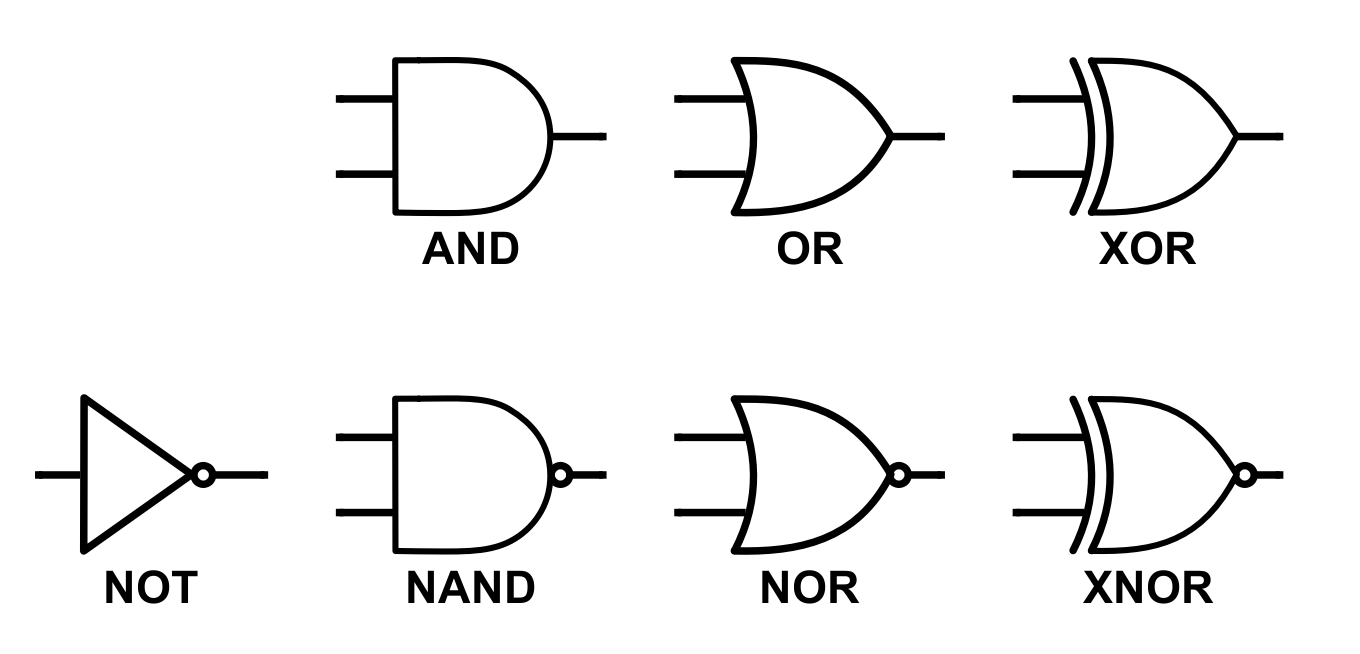
\includegraphics[width=10cm]{img/logic_gates.png}
	\caption{Simboli osnovnih logičkih vrata}
	\label{fig:logic-gates}
\end{figure}

Simboli logičkih vrata na slici \ref{fig:logic-gates} predstavljaju idealne elemente digitalne logike. Njihove realizacije u fizičkom svijetu građene su od poluvodičkih elemenata te su podložne zakonima fizike. Danas se logička vrata koriste kao dio integriranih krugova (engl.~\textit{integrated circuit}, IC) unutar čipova (engl.~\textit{chip}) izgrađenih od kristala silicija. Čipovi se kategoriziraju po svojoj složenosti tj.~broju logičkih vrata koje sadrže, od $10$ pa sve do stotine milijuna koliko ih se nalazi u modernim mikroprocesorima. Osnovni fizički elementi koji se realiziraju u strukturi silicija su diode i tranzistori. Dioda služi za propuštanje signala samo u jednom smjeru. Tranzistor je sličan diodi, ali se može upravljati količina propuštenog signala. Tranzistor je patentiran 1926.~godine i osnovni je element svih današnjih elektroničkih uređaja. Osnovna funkcija tranzistora jest pojačavanje signala tako da manji kontrolni signal upravlja protokom glavnog signala kroz tranzistor. Danas se najviše koristi MOS-FET (engl.~\textit{metal-oxide-semiconductor field-effect transistor}) izvedba tranzistora.

Postoji nekoliko ograničenja fizičkih elemenata koji grade digitalne sklopove. Prvo ograničenje jest vremensko kašnjenje odziva (engl.~\textit{propagation delay}). Ono proizlazi iz činjenice da kretanje električnog signala tj.~elektrona kroz vodič zahtijeva određeno vrijeme. Kašnjenje se može smanjiti skraćivanjem udaljenosti koju signal mora prijeći. Zato je razvoj modernih čipova usmjeren prema smanjenju pojedinih elemenata i vodiča koji ih spajaju. Drugo ograničenje jest faktor širenja (engl.~\textit{fan-out}) koji određuje maksimalan broj logičkih vrata koji se može spojiti na izlaz pojedinih vrata. Naime, logička vrata zahtijevaju određenu količinu električne struje kako bi se ulaz aktivirao. Svaka vrata koja se spoje na isti izlaz koriste dio raspoložive struje na tom ulazu te u jednom trenutku količina struje pada ispod praga aktivacije (engl.~\textit{activation threshold}). Treće ograničenje jest raspršenje energije (engl.~\textit{power dissipation}). Kretanje elektrona stvara toplinsku energiju koja se nakuplja u silicijevom kristalu. Potrebno je odvesti višak topline iz materijala jer će u suprotnom nastupiti degradacija materijala te će se izgubiti željena svojstva uređaja. Moderni mikroprocesori koriste CMOS (engl.~\textit{complementary} MOS) tranzistore koji troše malo energije kako bi se mogli gušće rasporediti u silicijevu rešetku.

\textbf{Multiplekser} (engl.~\textit{multiplexer}) je naziv za digitalni sklop koji služi za adresiranje ulaza. Multiplekser ima $2^{n}$ podatkovnih ulaza, $n$ adresnih ulaza te jedan izlaz. Adresa koja se nalazi na adresnim ulazima određuje indeks podatkovnog ulaza koji se preusmjerava na izlaz multipleksera. Na slici \ref{fig:mux-symbol} mogu se vidjeti dva multipleksera, prvi ima $n=1$ adresni ulaz i kraće se označava s $mux2/1$, dok drugi ima $n=2$ adresna ulaza i kraće se označava s $mux4/1$. Na slici \ref{fig:mux-gates} prikazan je $mux2/1$ ostvaren pomoću osnovnih logičkih vrata. Booleova funkcija koja se ostvaruje prikazana je izrazom \ref{eq:mux21} (zagrade nisu potrebne). Analogno tome definira se Booleov izraz za $mux4/1$ prikazan izrazom \ref{eq:mux41}. Multiplekseri se često koriste s demultiplekserima (engl.~\textit{demultiplexer}) koji obavljaju logički suprotnu funkciju: provođenje $1$ ulaza na neki od $2^{n}$ izlaza. Zajedno omogućavaju prijenos podataka preko jedne podatkovne linije.
%
\begin{align}
	\label{eq:mux21}
	Y_{2/1} &= (A \cdot \overline{S}) + (B \cdot S) \\
	\label{eq:mux41}
	Y_{4/1} &= (A \cdot \overline{S_{0}} \cdot \overline{S_{1}}) + (B \cdot S_{0} \cdot \overline{S_{1}}) + (C \cdot \overline{S_{0}} \cdot S_{1}) + (D \cdot S_{0} \cdot S_{1})
\end{align}

\begin{figure*}[htb]
	\subfloat[\label{fig:mux-symbol}]{
		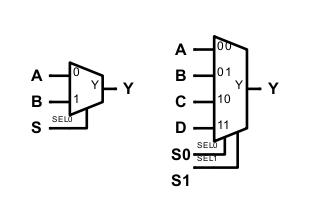
\includegraphics[width=0.4\textwidth]{img/mux_24_symbol.png}}
	\hspace{\fill}
	\subfloat[\label{fig:mux-gates}]{
		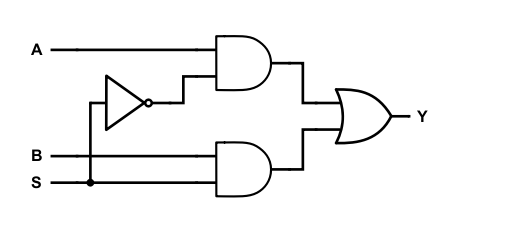
\includegraphics[height=0.267\textwidth]{img/mux_2_gates.png}}
	\caption{Prikaz multipleksera: (a) simboli (b) logička vrata}
	\label{fig:mux}
\end{figure*}

Za pohranu podataka u digitalnim sklopovima koriste se sklopke (engl.~\textit{latch}). Sklopke zadržavaju vrijednost na svom izlazu sve dok su opskrbljene strujom tj.~podaci se gube u slučaju da nestane struje. Najjednostavnija sklopka jest SR-sklopka (engl.~\textit{set-reset latch}) koja se može ostvariti sa samo $2$ NAND logička vrata. SR-sklopka ima nestabilna stanja (izlazna funkcija je nedefinirana za neke kombinacije ulaza) koja se uklanjaju uvođenjem kontrolnog signala. Rezultat je D-sklopka prikazana na slici \ref{fig:D-latch}. D-sklopka se može ostvariti s $4$ NAND logička vrata i $1$ inverterom (NOT). Ulaz D (engl.~\textit{data}) je podatkovni ulaz, a ulaz E (engl.~\textit{enable}) je kontrolni ulaz. Q i Q' su međusobno komplementarni izlazi. Impulsom na ulaz E sklopka zapamti vrijednost koja je u tom trenutku bila na D. Izlazi Q i Q' zadržavaju svoju vrijednost sve dok se impulsom na E ne dovede drugačija vrijednost s ulaza D. Karakteristični Booleov izraz za D-sklopku prikazan je izrazom \ref{eq:d-latch} gdje $n$ označava vremenski korak.
%
\begin{gather}
	\label{eq:d-latch}
	Q(n+1)=(E \cdot D) + (\overline{E} \cdot Q(n))
\end{gather}

\begin{figure}[htb]
	\centering
	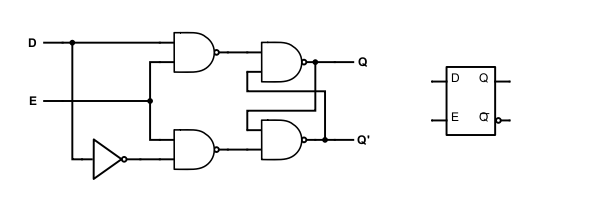
\includegraphics[width=0.9\textwidth]{img/D-latch_full.png}
	\caption{Prikaz D-sklopke}
	\label{fig:D-latch}
\end{figure}

\iffalse
\begin{figure*}[htb]
	\subfloat[\label{fig:d-latch-symbol}]{
		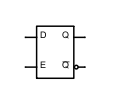
\includegraphics[width=0.24\textwidth]{img/D-latch_symbol.png}}
	\hspace{\fill}
	\subfloat[\label{fig:d-latch-gates}]{
		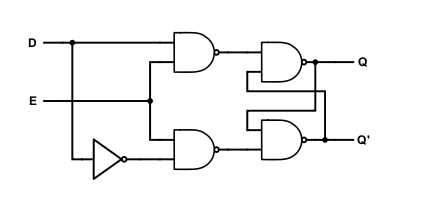
\includegraphics[width=0.66\textwidth]{img/D-latch_gates.png}}
	\caption{Prikaz D-sklopke: (a) simbol (b) logička vrata}
	\label{fig:D-latch}
\end{figure*}
\fi

D-sklopka može mijenjati svoj izlaz sve dok je signal E upaljen. To nastaje u problem u sekvencijskim digitalnim sklopovima (poput FPGA) gdje izlaz sklopke može negativno utjecati na njen ulaz. Zato se koristi signal takta (engl.~\textit{clock}) preko kojeg se sinkroniziraju sve promjene stanja. Kombinacijom $2$ D-sklopke i $1$ invertera nastaje \textbf{D-bistabil} (engl.~\textit{D flip-flop}) koji je prikazan na slici \ref{fig:D-flip-flop}. Promjena izlaza Q moguća je samo kada signal CLK prelazi iz $1$ u $0$. Tada se izlaz Y iz glavne (lijeve) D-sklopke upisuje u izlaz desne D-sklopke.
%
\begin{align}
	Y(n+1) &= (CLK \cdot D) + (\overline{CLK} \cdot Y(n)) \\
	Q(n+1) &= (\overline{CLK} \cdot Y(n+1)) + (CLK \cdot Q(n))
\end{align}

\begin{figure}[htb]
	\centering
	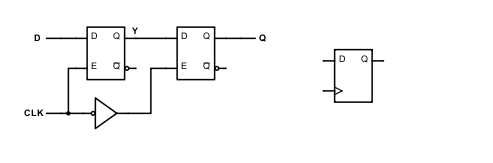
\includegraphics[width=0.9\textwidth]{img/D_flip-flop_full.png}
	\caption{Prikaz D-bistabila}
	\label{fig:D-flip-flop}
\end{figure}

\subsection{Potpuno binarno zbrajalo} \label{subsec:adders}

Potpuno binarno zbrajalo (engl.~\textit{full adder}) jest digitalni sklop koji zbraja $2$ binarne znamenke uzimajući u obzir vrijednost prijenosa (engl.~carry) na ulazu. Temeljni su dio aritmetičko logičkih jedinica (engl.~\textit{arithmetic logic unit}, ALU) u procesorima (engl.~\textit{central processing unit}, CPU). Jednostavnija verzija potpunog zbrajala jest poluzbrajalo (engl.~\textit{half adder}) koje nema ulaz za prijenos. Tablica \ref{tab:binary-addition} sadrži vrijednosti koje se dobiju pri potpunom zbrajanju binarnih znamenki $A$ i $B$. Neparan broj vrijednosti $1$ rezultira s $S=1$, dok više od jedne vrijednosti $1$ rezultira s $C_{OUT}=1$.

\begin{table}
	\centering
	\caption{Pravila zbrajanja binarnih znamenki}
	\label{tab:binary-addition}
	\begin{tabular}{|ccc|c|c|}
		\hline
		$A$ & $B$ & $C_{IN}$ 	& \hspace{0.29cm} $S$ \hspace{0.29cm} & $C_{OUT}$	\\
		\hline
		$0$ & $0$ & $0$			& $0$ & $0$			\\
		$0$ & $0$ & $1$			& $1$ & $0$			\\
		$0$ & $1$ & $0$			& $1$ & $0$			\\
		$0$ & $1$ & $1$			& $0$ & $1$			\\
		$1$ & $0$ & $0$			& $1$ & $0$			\\
		$1$ & $0$ & $1$			& $0$ & $1$			\\
		$1$ & $1$ & $0$			& $0$ & $1$			\\
		$1$ & $1$ & $1$			& $1$ & $1$			\\
		\hline
	\end{tabular}
\end{table}

Na slici \ref{fig:adders} prikazane su implementacije zbrajala pomoću logičkih vrata. Poluzbrajalo na slici \ref{fig:half-adder} koristi $1$ XOR vrata i $1$ AND vrata za ostvarenje izraza \ref{eq:half-adder-s} i \ref{eq:half-adder-c}. Dodavanjem ulaza za prijenos $C_{IN}$ dobiva se potpuno binarno zbrajalo čija  je implementacija pomoću logičkih vrata prikazana na slici \ref{fig:full-adder}. Potpuno zbrajalo koristi $2$ XOR vrata, $2$ AND vrata i $1$ OR vrata za ostvarenje izraza \ref{eq:full-adder-s} i \ref{eq:full-adder-c}.
%
\begin{align}
	\label{eq:half-adder-s}
	S &= A \otimes B \\
	\label{eq:half-adder-c}
	C &= A \cdot B \\
	\label{eq:full-adder-s}
	S &= A \otimes B \otimes C_{IN} \\
	\label{eq:full-adder-c}
	C_{OUT} &= (A \cdot B) + (C_{IN} \cdot (A \otimes B))
\end{align}

\begin{figure*}[htb]
	\subfloat[\label{fig:half-adder}]{
		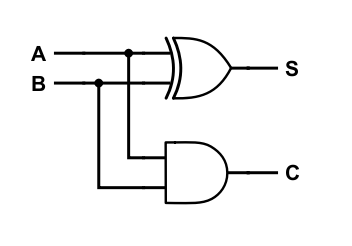
\includegraphics[width=0.3\textwidth, valign=t]{img/half_adder.png}
		\vphantom{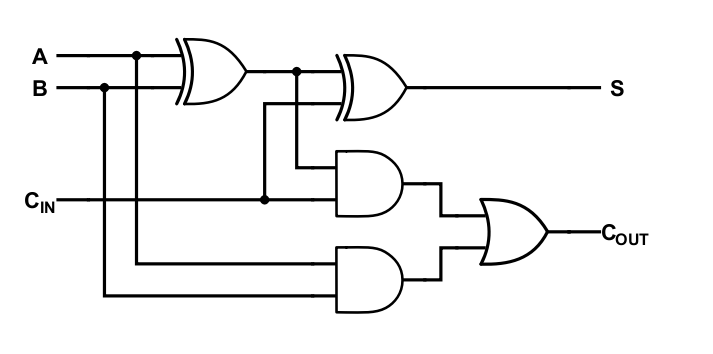
\includegraphics[width=0.5\textwidth, valign=t]{img/full_adder.png}}
	}
	\hspace{\fill}
	\subfloat[\label{fig:full-adder}]{
		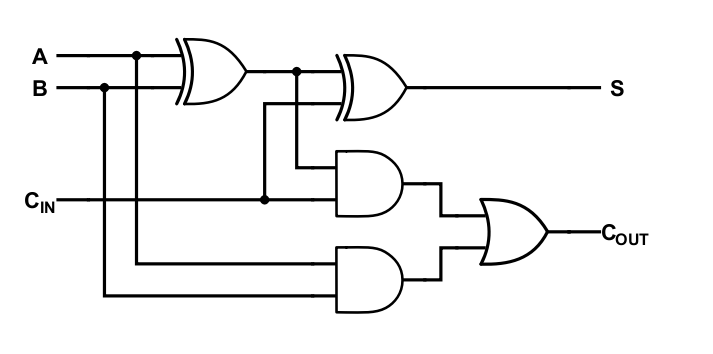
\includegraphics[width=0.6\textwidth, valign=t]{img/full_adder.png}}
	\caption{Binarna zbrajala: (a) poluzbrajalo (b) potpuno zbrajalo}
	\label{fig:adders}
\end{figure*}

Slaganjem više potpunih binarnih zbrajala u niz moguće je ostvariti zbrajanje višebitnih brojeva. Na slici \ref{fig:ripple-adder} prikazan je niz od $4$ međusobno ulančanih potpunih zbrajala (engl.~\textit{ripple carry adder}). Prvi binarni broj je $A_{3}A_{2}A_{1}A_{0}$, drugi binarni broj je $B_{3}B_{2}B_{1}B_{0}$, a izlaz je $S_{3}S_{2}S_{1}S_{0}$. $C_{IN}$ je ulazni prijenos, a $C_{3}$ je izlazni prijenos. Sva potpuna zbrajala (osim prvog) kao ulaz primaju prijenos od prethodnog zbrajala. Tako je za izračun izlazne vrijednosti $S_{3}$ potrebna vrijednost svih prethodnih prijenosa $C_{0}$, $C_{1}$ i $C_{2}$. Booleovi izrazi za izlazne funkcije dani su izrazima \ref{eq:ripple-adder-cin}, \ref{eq:ripple-adder-s} i \ref{eq:ripple-adder-c}. Prema slici \ref{fig:full-adder} $n$-bitno zbrajalo može se realizirati s $5n$ Booleovih funkcija dviju varijabli.
%
\begin{align}
	\label{eq:ripple-adder-cin}
	C_{-1} &= C_{IN} \\
	\label{eq:ripple-adder-s}
	S_{n} &= A_{n} \otimes B_{n} \otimes C_{n-1} \\
	\label{eq:ripple-adder-c}
	C_{n} &= (A_{n} \cdot B_{n}) + (C_{n-1} \cdot (A_{n} \otimes B_{n}))
\end{align}

\begin{figure}[htb]
	\centering
	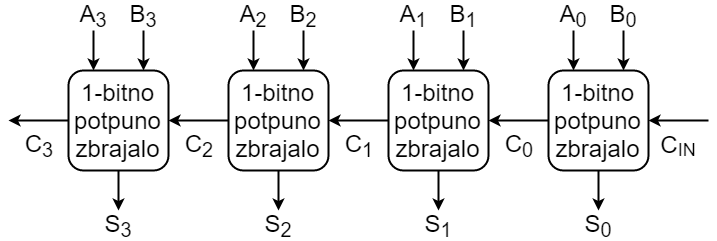
\includegraphics[width=0.9\textwidth]{img/ripple_adder.png}
	\caption{Prikaz D-bistabila}
	\label{fig:ripple-adder}
\end{figure}

\subsection{Konfigurabilni logički blokovi} \label{subsec:clb}

Konfigurabilni logički blokovi (engl.~\textit{configurable logic block}, CLB) predstavljaju osnovnu komponentu unutar FPGA. Na slici \ref{fig:clb} prikazana je osnovna struktura CLB-a s $3$ ulaza. Blok se sastoji od \textbf{pregledne tablice} (engl.~\textit{look-up table}, LUT), multipleksera tablice (na slici lijevo), D-bistabila te izlaznog multipleksera (na slici desno) s pripadnom tablicom koja sadrži samo jednu vrijednost $S$. CLB ima $3$ funkcijska ulaza $\{A, B, C\}$, ulaz za sinkronizacijski takt $CLK$ te izlaz $Y$. CLB može implementirati bilo koju Booleovu funkciju s istim ili manjim brojem ulaza. To se jednostavno postiže upisom tablice istinitosti željene Booleove funkcije u preglednu tablicu. Za realizaciju pregledne tablice koristi se memorija. Najčešće se koristi SRAM (engl.~\textit{static random-access memory}) zbog svoje brzine i jednostavnosti sklopovlja. Na primjer, DRAM (engl.~\textit{dynamic RAM}) koja se koristi za glavnu memoriju u računalima puno je jeftinija za isti kapacitet, ali zahtijeva posebno sklopovlje za osvježavanje \cite{book:memory}. D-bistabil i izlazni multiplekser koriste se za izbor načina rada. Upisivanjem vrijednosti $0$ u $S$, na izlaz se direktno dovodi izlaz iz funkcijskog multipleksera. Kaže se da CLB radi u asinkronom načinu rada bez obzira na sinkronizacijski takt $CLK$. Upisivanjem vrijednosti $1$ u $S$, na izlaz se dovodi podatak spremljen u D-bistabilu (njegov izlaz $Q$). Pritom se u D-bistabil sprema vrijednost izlaza funkcijskog multipleksera na negativan brid od $CLK$ (kada prijeđe iz $1$ u $0$). Kaže se da CLB radi u sinkronom načinu rada i izlaz $Y$ mijenja se samo pri promjeni takta $CLK$. Kod CLB-ova s više ulaza često se pregledna tablica i pripadajući multiplekser implementiraju s više manjih komponenti.

\begin{figure}[htb]
	\centering
	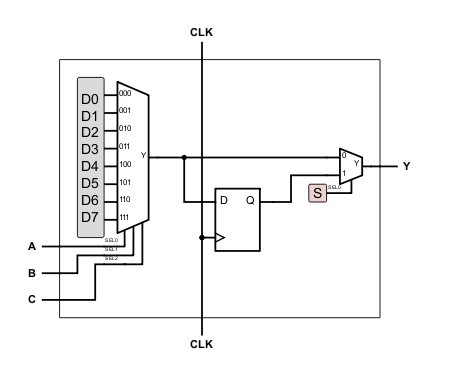
\includegraphics[width=0.8\textwidth]{img/CLB.png}
	\caption{Struktura CLB-a s $3$ ulaza}
	\label{fig:clb}
\end{figure}

Za izvršavanje algoritama postoje dvije krajnje mogućnosti \cite{article:reconfigurable}. Prva mogućnost su računala s mikroprocesorima. Algoritam se unese u računalo, tipično uporabom programskih jezika, nakon čega se algoritam izvodi koristeći skup instrukcija podržanih od strane procesora. Prednosti su jednostavnost i mala cijena razvoja. Jednostavnost je rezultat više razina apstrakcije koje moderni programski jezici nude (poput programskog jezika Java). Programeru jest omogućena implementacija složenih algoritama bez potrebe za znanjem o detaljima arhitekture računalnog sustava. Mala cijena proizlazi iz primjenjivosti na modernim računalima koja su univerzalna te se proizvode u velikim serijama. Algoritam se može izvoditi na više procesora, može se izvoditi paralelno uz druge zadaće, itd.

Druga mogućnost jest izrada posebnog digitalnog sustava koji će implementirati željenu funkcionalnost tj.~algoritam. Konkretno, može se koristiti ASIC (engl.~\textit{application-specific integrated circuit}). To je integrirani krug koji se dizajnira i proizvodi za specifičnu namjenu. Današnji ASIC čipovi sadrži stotine milijuna logičkih vrata te može sadržavati procesore, memoriju i slične blokove složenih funkcionalnosti. U tom slučaju koristi se naziv "sustav na čipu" (engl.~\textit{system-on-chip}). Najveća prednost ASIC-a jest u brzini izvođenja. Direktno korištenje logičkih vrata za potrebe izvođenja algoritma puno je brže od izvođenja na mikroprocesorima. Razlog tome jest što mikroprocesor slijedno odrađuje instrukcije te troši vrijeme na dekodiranje svake instrukcije i pristup memoriji. Iako moderna računala imaju nekoliko jezgri od kojih svaka može odrađivati više instrukcija odjednom, mogućnost paralelizacije na razini logičkih vrata puno je veća. Unatoč tome, korištenje posebnih čipova ima veliki nedostatak. Naime, razvoj i cijena pokretanja proizvodnje su jako skupi te mogu doseći milijune američkih dolara. Zato se danas većinom koriste samo za veliku serijsku proizvodnju. Primjer uspješne primjene ASIC-a su uređaji za "rudarenje" kriptovaluta poput Bitcoina. Takvi uređaji su puno učinkovitiji od alternativa poput grafičkih kartica (engl.~\textit{graphics processing unit}, GPU) jer troše puno manje struje koja predstavlja najveći trošak.

FPGA tehnologija služi kao srednja opcija između brzine ASIC-a i univerzalnosti mikroprocesora. Na slici \ref{fig:fpga_island} prikazana je osnovna struktura FPGA uređaja, tzv.~otočni raspored (engl.~\textit{island style}). Elementi su poslagani u dvodimenzionalno polje, a između ćelija se prostiru linije za prijenos signala. Ovo je najčešće korišteni raspored jer nudi visok stupanj fleksibilnosti. Postoje i drugi rasporedi kao što je raspodjela elemenata u stupce između kojih se nalaze sabirnice. Međutim, praktična primjena je pokazala da je dobra povezanost elemenata ključna za performanse uređaja. Zato se danas većina prostora na FPGA čipu koristi za resurse povezivanja (oko $60\%$ pa čak i do $90\%$).

\begin{figure}[htb]
	\centering
	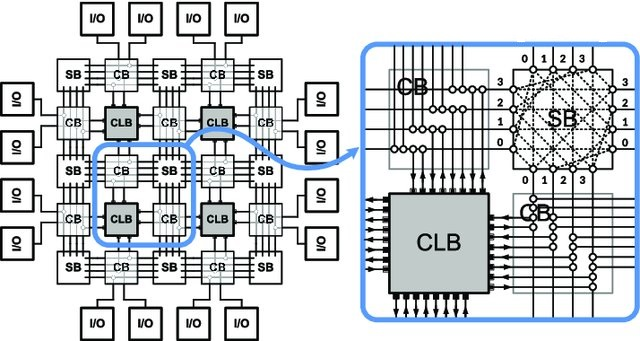
\includegraphics[width=0.8\textwidth]{img/fpga_island_notext.jpg}
	\caption{Raspored elemenata u FPGA}
	\label{fig:fpga_island}
\end{figure}

FPGA uređaj na periferiji sadrži veći broj \textbf{ulazno-izlaznih blokova} (engl.~\textit{input-output block}, IOB) koji služe za komunikaciju uređaja s okolinom. Blok se konfigurira kao ulazni, izlazni ili oboje istovremeno. Ulazi i izlazi se sastoje od jedne binarne vrijednosti, ali je moguće po potrebi koristiti više blokova. FPGA radi na određenom taktu koji određuje vrijeme koje je potrebno da uređaj pročita ulaze te izračuna potrebne izlaze. Radna frekvencija ovisi o najduljem putu između međusobno povezanih elemenata. Za konfiguraciju FPGA potrebno je upisati podatke u memorijske elemente te aktivirati ili ugasiti poluvodičke elemente koji služe kao osigurači (engl.~\textit{fuse}). Na programskoj razini to odgovara stvaranju posebne datoteke koja sadrži niz bitova (engl.~\textit{stream}). Konfiguracija je brza i izvodi se prije svakog pokretanja uređaja. Napredniji uređaju podržavaju rekonfiguraciju tj.~konfiguraciju dijela (ili cijelog) uređaja tijekom rada.

Signali unutar FPGA putuju po spojnim linijama koje su raspoređene u mrežu po redcima i stupcima. Na raskrižjima se nalaze \textbf{prespojne kutije} (engl.~\textit{switch box}, SB) koje služe za preusmjeravanje signala. Postoji više usporednih spojnih linija između susjednih prespojnih kutija. Uređaji često sadrže spojne linije raznih duljina koje mogu "preskakati" određeni broj spojnih kutija. Razlog njihova korištenja jest ubrzanje rada uređaja. Naime, spojevi unutar prespojnih kutija imaju puno veće kašnjenje u odnosu na neprekinuti vodič. Često postoji potreba za globalnim signalima unutar uređaja za što se koriste spojne linije koje se protežu cijelom širinom ili duljinom uređaja. U gornjem desnom dijelu slike \ref{fig:fpga_island} mogu se vidjeti moguće kombinacije prespajanja unutar jedne spojne kutije. Spojne linije označene su brojevima $\{0, 1, ..., n-1\}$. Svaka linija može biti spojena s $3$ pripadajuće linije na ostale $3$ strane spojne kutije. Broj mogućih spojeva bez preskakivanja prikazan je izrazom \ref{eq:sb-combinations} što za spojnu kutija sa slike \ref{fig:fpga_island} iznosi $6n = 24$ \cite{article:switch_box}. Korištenjem preskakivanja spojnih linija, broj mogućnosti može se smanjiti na $n$. Pritom broj mogućih konfiguracija prespojne kutije drastično pada.
%
\begin{gather}
	\label{eq:sb-combinations}
	\frac{broj\_strana * broj\_linija * (broj\_strana - 1)}{dupli\_bridovi} = \frac{4 * n * 3}{2} = 6n
\end{gather}

Unutar mreže prespojnih elemenata nalaze se logički elementi, a najčešće su to konfigurabilni logički blokovi. Osnovna struktura CLB-a objašnjena je u odjeljku \ref{subsec:clb}. Svaki logički element okružen je spojnim blokovima (engl.~\textit{connector block}, CB). Oni omogućavaju povezivanje logičkog elementa sa spojnim linijama. Često postoje direktne linije između susjednih logičkih elemenata kako bi se rasteretile spojne linije i smanjilo kašnjenje signala. Moderni FPGA uređaji poput Xilinx Virtex 7 sadrže razne gotove (ne konfigurabilne) elemente uz CLB-ove. Uređaj je podijeljen na više jednakih područja od kojih se svaki sastoji od većeg broja CLB-ova i više dodatnih elemenata. Najčešće su to razne vrste memorije. Iako je moguće pomoću kaskade CLB-ova konfigurirati memoriju proizvoljne veličine (uz dovoljan broj blokova), dodavanjem konkretnih memorijskih elemenata troši se manje prostora na uređaju te se postiže brži pristup podacima. Još jedna često korištena funkcija koja se teže implementira CLB-ovima jest operacija množenja. Raspodjelom takvih elemenata po uređaju osigurava se kraći put do CLB-ova. Dodatne mogućnosti uključuju integrirane mikroprocesore, kontrolnu logiku (npr. FIFO) i ispravljanje pogrešaka (engl.~\textit{error correcting code}, ECC).

%%%%%
%%%%%
%%%%%

\section{Problem dekompozicije} \label{sec:decomposition}

Problem koji se ovdje razmatra jest kako skup Booleovih funkcija tj.~vektorsku Booleovu funkciju (u nastavku Booleov vektor) implementirati u tehnologiji FPGA korištenjem što manjeg broja konfigurabilnih logičkih blokova (CLB). Motivacija je jednostavna, manjim brojem CLB-ova troši se manje resursa i uređaj radi brže. Problem nastaje kada je broj ulaza $n$ Booleove funkcije veći od broja ulaza $m$ CLB-a pri čemu je onda potrebno iskoristiti više CLB-ova za njenu implementaciju. Kako CLB s $m$ ulaza može implementirati bilo koju Booleovu funkciju s $m$ ulaza onda je problem istovjetan problemu pronalaska podfunkcija $f_{i}$ koje čine dekompoziciju glavne funkcije $f$. Pritom je potrebno prepoznati zajedničke podfunkcije ako one postoje te ih zasebno (bez ponavljanja) realizirati pomoću CLB-ova. Krajnje rješenje sadržavalo bi CLB-ove koji se koriste u izračunu više funkcija. Time bi se povećala iskoristivost blokova i smanjila redundantnost u izračunu izlaza.

Navedeni problem je kombinatorički složen te ne postoje algoritmi koji garantiraju optimalno rješenje u razumnom vremenu. Moguće je konstruirati rješenje koristeći "grubu silu" (engl.~\textit{brute force}) i iterirati kroz sve moguće kombinacije CLB-ova, ali ovakav pristup nije praktičan. Razlog tome jest \textbf{kombinatorička eksplozija} tj.~broj kombinacija raste eksponencijalno u odnosu na broj blokova (oznaka $n$). Eksponencijalna vremenska ovisnost još se označava s $O(c^{n})$ (engl.~\textit{big O notation}) gdje je $c$ konstanta (najčešće $2$). U sklopu računarske znanosti takvi se problemi nazivaju \textbf{NP problemi} (engl.~\textit{nondeterministic polynomial time}). To su problemi koji se teško računaju za razliku od problema čija se rješenja mogu izračunati u polinomijalnom vremenu (oznaka P). Rješavanje ovakvih problema svodi se na korištenje algoritama koji nalaze što bolje rješenje u razumnom vremenu. Ne postoji garancija da je dobiveno rješenje optimalno, ali zato je često vrlo blizu optimalnom rješenju.

%%%%%
%%%%%
%%%%%

\chapter{Implementacija rješenja} \label{chapter:impl}

U ovom poglavlju opisana je implementacija rješenja problema objašnjenog u odjeljku \ref{sec:decomposition}. Detaljan opis razvijenog algoritma dan je u odjeljcima \ref{subsec:implementation} i \ref{subsec:solver}. Njima prethodi objašnjenje pojma heuristike uz kratak pregled teorije korištenih heuristika. U svrhu lakšeg korištenja samog algoritma, razvijeno je i jednostavno grafičko sučelje. Odjeljak \ref{sec:gui} opisuje osnove korištenja grafičkog sučelja te nudi popis podržanih funkcionalnosti. Cjelokupna implementacija izvedena je u programskom jeziku Java. To je objektno orijentirani programski jezik i platformski je neovisan. Izvorni kod napisan u Javi prevodi se u Java Bytecode koji se pokreće Javinoj virtualnoj mašini (engl.~\textit{Java Virtual Machine}, JVM). Osim standardnih biblioteka, korištena je i biblioteka Gson koja služi za učitavanje i zapis podataka u JSON formatu (engl.~\textit{JavaScript Object Notation}). Grafičko sučelje razvijeno je pomoću standardne biblioteke Swing. Ona sadrži skup alata i gotovih komponenti koje omogućuju brži razvoj jednostavnih sučelja.

%%%%%
%%%%%
%%%%%

\section{Postupak dekompozicije} \label{sec:impl_decomp}

Kao što je već objašnjeno u odjeljku \ref{sec:decomposition}, postupak dekompozicije Booleove funkcije vrlo je složen. To je optimizacijski problem za kojeg postoji veći broj rješenja, a samo jedno od njih (ili nekoliko) je najbolje. Općenito, rješavanje optimizacijskog problema svodi se na pronalazak najboljeg rješenja. Prvi korak jest identifikacija problema što je već napravljeno u odjeljku \ref{sec:decomposition}. Preostala dva koraka su: modeliranje problema i optimizacija problema. Njihova implementacija može imati $2$ smjera. Prva opcija prikazana je izrazom \ref{eq:option1}. Koristi se model koji pojednostavljuje neke dijelove problema i pokušava ga se optimizirati s egzaktnim algoritmom optimizacije. Prednost ovakvog pristupa jest što se garantira pronalazak optimalnog rješenje u razumnom vremenu, ali to rješenje odnosi se na pojednostavljeni model. Primjeri egzaktnih algoritama su: dinamičko programiranje, simpleks metoda te metoda grananja i granica (engl.~\textit{branch and bound}). Druga opcija prikazana je izrazom \ref{eq:option2}. Koristi se model koji precizno opisuje problem i pokušava ga se optimizirati s aproksimativnim algoritmom. Prednost jest što se u obzir uzimaju svi zahtjevi problema, ali ne postoji garancija da je algoritam pronašao optimalno rješenje.
%
\begin{gather}
	\label{eq:option1}
	problem \rightarrow model_{jednostavan} \rightarrow rjesenje_{egzaktno}(model_{jednostavan}) \\
	\label{eq:option2}
	problem \rightarrow model_{precizan} \rightarrow rjesenje_{aproks.}(model_{precizan})
\end{gather}

U nastavku će se razmatrati druga opcija tj.~korištenje aproksimativnog algoritma za rješavanje preciznog modela. Kao naziv takvih algoritama koristi se pojam "heuristika". Naziv dolazi od starogrčke riječi \textit{heuriskein} za umijeće pronalaska novih strategija za rješavanje problema. Pritom se optimizacijski problem definira kao dvojka $P=(S,f)$ gdje je $S$ skup svih mogućih rješenja, a $f:S \mapsto \Re$ predstavlja funkciju cilja koju treba optimizirati. Optimizacija funkcije cilja svodi se na pronalazak njenog \textbf{globalnog optimuma} $s^{*} \in S$ za kojeg vrijedi $f(s^{*}) \leq f(s), \forall s \in S$ (minimizacija), odnosno $f(s^{*}) \geq f(s), \forall s \in S$ (maksimizacija). Na slici \ref{fig:optimum} prikazan je primjer funkcije cilja. Funkcija ima $3$ lokalna optimuma od kojih je samo jedan globalni optimum $s^{*}$. Problem predstavljaju područja označena žutom bojom. Kako bi algoritam došao iz jednog od lokalnih optimuma $s'$ u globalni optimum $s^{*}$ on mora pretraživati u smjeru lošijih rješenja kao što je prikazano strelicama.

\begin{figure}[htb]
	\centering
	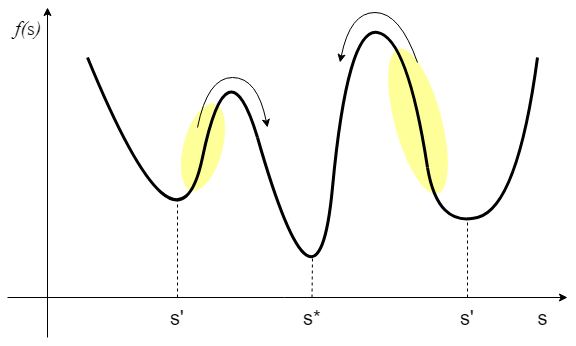
\includegraphics[width=0.6\textwidth]{img/optimum.png}
	\caption{Globalni i lokalni optimum}
	\label{fig:optimum}
\end{figure}

Heuristički algoritmi dijele se u $2$ kategorije: konstruktivne heuristike i poboljšavajuće heuristike. Konstruktivne heuristike evaluiraju parcijalna rješenja i u koracima izgrađuju konačno rješenje. Primjer su pohlepni algoritmi. Poboljšavajuće heuristike još se nazivaju \textbf{metaheuristike} od grčke riječi \textit{meta} za metodologiju višeg sloja. Naziv su dobile po tome što su, uz određene prilagodbe, primjenjive na bilo koji optimizacijski problem. Proces prilagodbe tj.~krojenja heuristike za rješavanje određenog problema zapravo je optimizacijski problem sam po sebi. Heuristika se sastoji od strategije i određenog broja parametara koji se još nazivaju hiperparametri. Potrebno je odabrati one parametre za koje heuristika daje najbolje rezultate. Nerijetko je to mukotrpan proces koji uvelike ovisi o iskustvu i intuiciji inženjera. Srećom, postoje već gotovi "recepti" za mnoštvo postojećih problema, dok se novi problemi često mogu svesti na postojeće problema. Većina metaheuristika oponaša prirodne fenomene po kojima su dobila nazive. Primjeri metaheuristika su: lokalno (engl.~\textit{local search}) i tabu pretraživanje (engl.~\textit{tabu search}), simulirano kaljenje, genetski algoritam i algoritam mravlje kolonije (engl.~\textit{ant colony optimization}). Heuristike mogu biti stohastičke što znači da iz istog početnog stanja mogu doći do različitih rješenja.

\subsection{Genetski algoritam}

Genetski algoritam (engl.~\textit{genetic algorithm}) je stohastička metaheuristika koja oponaša prirodni fenomen evolucije \cite{book:evolution}. Prva inačica genetskog algoritma nastala je 1960-ih godina. Strategija algoritma jest natjecanje između jedinki. Svaka jedinka je potencijalno rješenje optimizacijskog problema. Algoritam počinje od početne populacije (skup jedinki) te iterativno pokušava poboljšati jedinke u populaciji. Broj jedinki u populaciji jest parametar koji se naziva "veličina populacije". Pojedine iteracije zovu se generacije. Stvaranje početne populacije jedinki zove se inicijalizacija i najčešće se izvodi nasumično. Nad jedinkama se koriste $3$ vrste operatora: selekcija (engl.~\textit{selection}), križanje (\textit{crossover}) i mutacija (engl.~\textit{mutation}). Pritom je potrebno pridržavati se $2$ suprotna kriterija. Prvi kriterij jest \textbf{eksploatacija} (engl.~\textit{exploitation}) tj.~iskorištavanje najboljih jedinki. Eksploatacija odgovara približavanju lokalnom optimumu funkcije cilja. Drugi kriterij jest \textbf{diverzifikacija} (engl.~\textit{diversification}) tj.~istraživanje područja rješenja. Naime, algoritam može "zapeti" u lokalnom optimumu tj.~rješenje koje daje ne odgovara globalnom optimumu kojeg se želi naći. Razlog tome jest što početna populacija ne mora sadržavati prostor u kojem se nalazi globalni optimum. Eksploatacija daljnje sužava prostor pretraživanja i zanemaruje lošija rješenja koja se nalaze na putu do globalnog optimuma. Zato je važno ugraditi određenu količinu nasumičnosti u algoritam kako bi uzimao u obzir putove koji se na prvi pogled čine lošijima.

Operator selekcije odabire $2$ jedinke iz populacije na temelju njihove kvalitete (engl.~\textit{fitness}). Cilj selekcije jest oponašati prirodnu selekciju tj.~preživljavanje najboljih. Jedinke koje imaju veći \textit{fitness} imaju veće šanse da budu odabrane. $2$ odabrane jedinke postaju roditelji koji će sudjelovati u križanju. Postoji više mogućih implementacija operatora selekcije. Može se koristiti odabir jedinki proporcionalno njihovoj kvaliteti (engl.~\textit{roulette-wheel selection}). Jedinke se prvo sortiraju po kvaliteti. Zatim se izračuna kumulativni \textit{fitness} za svaku jedinku tako što joj se pribroji \textit{fitness} svih prethodnih. Pritom se zbroj svih kumulativnih vrijednosti mora normalizirati na vrijednost $1$. Odabir se izvodi nasumičnim brojem u rasponu $r \in [0, 1]$ te odabirom prve jedinke za koju je kumulativan \textit{fitness} veći ili jednak $r$. Može se primijetiti da je ovaj postupak računski zahtjevan zbog sortiranja i iteriranja. Operatori u genetskom algoritmu izvode se velik broj puta te je poželjno da su brzi. Zato se češće koristi stohastička (nasumična) verzija koja daje slične rezultate. To je \textbf{turnirska selekcija} (engl.~\textit{tournament selection}), a postupak je jednostavan: nasumično se odabere $n$ jedinki te se odabere najkvalitetnija. Pritom parametar "veličine turnira" $n$ određuje "selekcijski pritisak" (engl.~\textit{selection pressure}).  Kvalitetnije jedinke imaju veće šanse za "pobijediti" u turniru kako se veličina turnira povećava. Potrebno je napomenuti još jedan važan pojam kod evolucijskih algoritama. \textbf{Elitizam} je mehanizam automatskog prosljeđivanja najboljih jedinki u sljedeću generaciju bez promjena. Ovime se garantira da algoritam neće "zaboraviti" trenutno najbolje rješenje (engl.~\textit{incumbent solution}). Broj najboljih jedinki koji se sačuva jest parametar koji se naziva "veličina elitizma".

Operator križanja jest najvažniji genetski operator. Križanjem $2$ jedinke (roditelji) nastaju $2$ nove jedinke (njihova djeca). Prvo je potrebno odrediti format genetske informacije tj.~podataka koji određuju jedinku. Tu se mogu razlikovati genotip i fenotip. Genotip je naziv za konkretne podatke spremljene unutar računala. Način pohrane je proizvoljan, a najčešće se koriste nizovi bitova. Fenotip je naziv za interpretaciju genotipa jedinke. Točnije, fenotip je preslikavanje iz genotipa u rješenje. Na primjer, kod traženja minimuma funkcije genotip može biti niz vrijednosti parametara funkcije. Primjer genotipa za funkciju $3$ varijabli je $\{5, 13, 6\}$. Fenotip je pridruživanje tih brojeva pripadajućim varijablama. Primjer fenotipa je $\{x=6, y=13, z=5\}$ (obrnuti redoslijed). Ovdje će se koristiti nizovi cijelih brojeva koji će predstavljati stablo CLB-ova. Oblik genotipa može uvelike utjecati na svojstva algoritma. Za primjer se može uzeti problem dodjeljivanja $n$ prostorija među $m$ predavača. Binarni genotip odgovarao bi dvodimenzionalnom polju gdje vrijednost elementa $p_{ij}=\{0, 1\}$ govori je li prostorija $i$ dodijeljena predavaču $j$. Takvo polje bilo bi dimenzija $n \times m$ što potencijalno može zauzimati puno memorije. Drugi način jest koristiti cjelobrojni genotip duljine $m$ gdje bi vrijednost $p_{j}=i$ govorila koja prostorija je dodijeljena $j$-tom predavaču.

Križanjem se izvodi rekombinacija genotipa. Dijete naslijedi dio genotipa od prvog roditelja, a ostatak genotipa naslijedi od drugog roditelja. Drugo dijete naslijedi preostale dijelove genotipa. Najjednostavniji način križanja jest \textbf{križanje s prekidnim točkama}. One dijele genotip na dijelove. Na slici \ref{fig:crossover} može se vidjeti križanje s $2$ prekidne točke. Prekidne točke se odabiru nasumično i iste su za oba roditelja. Djeca redom naizmjenično nasljeđuju dijelove genotipa. Broj prekidnih točaka i razmak između njih su parametri. Još jedan primjer jest jednoliko križanje (engl.~\textit{uniform crossover}). Genotip se dijeli na najmanje dijelove (najčešće na razini bitova) te su jednake šanse za naslijediti dio iz jednog od roditelja. Navedena križanja su jednostavna te mogu rezultirati jedinkom koja nije valjana tj.~ne ispunjava uvjete optimizacijskog problema. U tom slučaju potrebno je više puta pokušavati križanje ili koristiti "pametnije" operatore križanje.

\begin{figure}[htb]
	\centering
	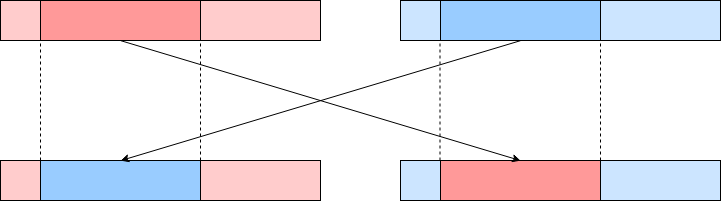
\includegraphics[width=0.6\textwidth]{img/crossover.png}
	\caption{Križanje s $2$ prekidne točke}
	\label{fig:crossover}
\end{figure}

Operator mutacije uvodi malenu promjenu u genotipu jedinke. Mutiraju se djeca dobivena križanjem. Time se unose "svježi geni" u populaciju s ciljem diverzifikacije. Mutacija većinom vremena smanjuje kvalitetu jedinke, ali to nije problem. Ono što je važno jesu rijetke mutacije koje unaprijede (najbolje) rješenje. One su potrebne za pronalazak boljih rješenja koja se ne mogu dobiti nikakvom kombinacijom križanja već prisutnih jedinki. Vrlo je važno koristiti malen parametar vjerojatnosti mutacije jer velik broj mutacija degradira algoritam u nasumičnu potragu. Jednostavan primjer mutacije jest jednolika mutacija (engl.~\textit{uniform mutation}). Za svaki dio genotipa postoji malena vjerojatnost da će se promijeniti.

Genetski algoritam ne može znati ako je našao najbolje rješenje pa je zato potreban \textbf{kriterij zaustavljanja} (engl.~\textit{termination criteria}). Postoji više mogućih načina za odrediti uvjet zaustavljanja. Najčešće se koristi više kriterija istovremeno te algoritam prestaje s radom čim se ispuni neki od njih. Najčešće korišteni kriterij odnosi se na vremensko ograničenje izvođenja. Osim vremenom, kriterij zaustavljanja može biti definiran s najvećim dozvoljenim brojem generacija. Broj generacija odgovara određenoj količina "posla" koju genetski algoritam mora izvesti pa se smanjuje ovisnost o brzini izvođenja. Još jedna mogućnost jest praćenje kvalitete najbolje jedinke. Može se odrediti prag kvalitete jedinke pa će genetski algoritam stati čim pronađe jedinku s jednakom ili većom kvalitetom od zadanog praga. Pamćenjem kvalitete najbolje jedinke kroz više generacija, moguće je prepoznati stagniranje i zaustaviti izvođenje. Pretpostavka je da daljnja pretraga nije isplativa pa se uštedi na vremenu.

Jedna od naprednijih mogućnosti jest \textbf{paralelizacija genetskog algoritma}. Vrijeme izvođenja predstavlja jedno od najvećih ograničenja prilikom rješavanja optimizacijskih problema. Paralelizacijom se ubrzava izvođenje tako što se koristi više računalnih resursa. Moderni računalni sustavi sadrže veći broj procesorskih jezgri od kojih svaka može izvoditi nekoliko programa odjednom. Programi se izvode na logičkim dretvama (engl.~\textit{thread}) unutar procesora. Potrebno je omogućiti izvođenje algoritma u višedretvenom okruženju što često predstavlja izazov. Pogrešnom komunikacijom između dretvi može doći do neočekivanih problema koji se ne pojavljuju u jednodretvenom izvođenju. Komunikacija je potrebna pri pristupanju dijeljenim podacima pri čemu postoje dva pristupa. Prvi pristup jest korištenje zasebnih populacija između kojih jedinke mogu "migrirati". Nije potrebno sinkronizirati jedinke unutar populacija, ali je zato ograničeno križanje jedinki iz različitih populacija. Drugi pristup jest dijeljenje jedne populacije pri čemu svaka dretva obrađuje jedan dio populacije. Potrebna je veća razina kontrole izvođenja, ali je moguće križati bilo koji par jedinki.

U nastavku je pseudokod jednostavne inačice genetskog algoritma. Uklanjanjem $2$ jedinke na kraju postoji mogućnost da će se izbaciti dobivena djeca. Time se odbacuju nova rješenja koja su lošija od ostatka populacije.

\begin{algorithm}
	\SetKwFunction{init}{inicijalizacija}
	\SetKwFunction{eval}{evaluiraj}
	\SetKwFunction{operSelect}{selekcija}
	\SetKwFunction{operCrossover}{križanje}
	\SetKwFunction{operMutate}{mutacija}
	{
		populacija = \init{}\;
		\eval{populacija}\;
		\While{uvjet\_zaustavljanja}{
			roditelji = \operSelect{populacija}\;
			djeca = \operCrossover{roditelji}\;
			\operMutate{djeca}\;
			\eval{djeca}\;
			populacija += djeca\;
			izbaci $2$ najgore jedinke iz populacije\;
		}
	}
	\caption{Osnovni genetski algoritam}
\end{algorithm}

\subsection{Lokalno pretraživanje i simulirano kaljenje}

Lokalno pretraživanje (engl.~\textit{local search}) je jednostavna deterministička metaheuristika koja ne imitira prirodne fenomene. Ideja jest raditi malene promjene u rješenju te tako malim koracima poboljšavati rješenje. Lokalno pretraživanje jest generički pristup rješavanja te se često koristi u sklopu ostalih heuristika kao što je simulirano kaljenje. Lokalno pretraživanje definira susjedstvo $N(s) \subset S$ rješenja $s$ kao podskup skupa svih rješenja $S$. Svaki susjed $s' \in N(s)$ jest rješenje koje se može dobiti iz trenutnog stanja $s$ uz dovoljno malen pomak. Funkcija susjedstva je mapiranje $n(s): S \mapsto 2^{S}$ za koje postoje $2$ glavne strategije: nasumična pretraga i pohlepna pretraga. Nasumična pretraga generira manje susjedstvo pa je brža, ali zato sporije konvergira. Pohlepna pretraga generira veće susjedstvo pa je sporije, ali zato brže konvergira.

Simulirano kaljenje (engl.~\textit{simulated annealing}) je stohastička metaheuristika koja imitira prirodni fenomen kaljenja materijala. Razvijena je 1980-ih godina na temelju Monte Carlo modela. Prirodni proces kaljenja najčešće se koristi pri termičkoj obradi metala. Metal se zagrijava te se potom sporo hladi. Početna temperatura ne smije biti previsoka i hlađenje ne smije biti prebrzo. Kristalna rešetka unutar metala polako prelazi iz stanja visoke energije (užareni metal) u stanje niske energije (hladan metal). Ovaj proces polako raspoređuje atome unutar kristalne rešetke u veće kristale s puno jačim vezama između atoma. Rezultat je puno čvršći materijal. Algoritam simuliranog kaljenja na sličan način koristi parametar topline.

Koristi se samo jedna jedinka za razliku od genetskog algoritma koji koristi populaciju. Algoritam iterativno pronalazi susjedno rješenje u koje prelazi ovisno o kvaliteti rješenja $f(s)$ te o trenutnoj vrijednosti temperature (oznaka $T$). Vjerojatnost prihvaćanja lošijeg rješenja ovisi o funkciji prihvaćanja $P(\Delta f, T)$ prema izrazu \ref{eq:sa-accept1} gdje $\Delta f=f(susjed)-f(trenutno)$ (problem minimizacije) predstavlja razliku kvalitete trenutnog i susjednog rješenja. Izraz \ref{eq:sa-accept1} odgovara Boltzmannovoj distribuciji iz termodinamike (za $k=1$ je $kT=T$ u nazivniku). Poboljšavajuća rješenja se uvijek prihvaćaju. Alternativna tome jest uvijek prihvaćati susjedno rješenje uz određenu vjerojatnost. U tom slučaju koristi se izraz \ref{eq:sa-accept2}. Jednaka je vjerojatnost za odbijanje puno lošijih i puno boljih rješenja, ali u prosjeku je puno više lošijih susjeda pa algoritam bolje radi.
%
\begin{gather}
	\label{eq:sa-accept1}
	P(\Delta f, T)=\exp(\frac{- \Delta f}{T}) \\
	\label{eq:sa-accept2}
	P(\Delta f, T)=\frac{1}{1 + \exp(\frac{\Delta f}{T})} \\
	\label{eq:sa-limit-upper}
	\lim_{T \to \infty} P(\Delta f, T)=1 \\
	\label{eq:sa-limit-lower}
	\lim_{T \to 0} P(\Delta f, T)=0
\end{gather}

Temperatura $T$ na početku ima visoku vrijednost pa se prema izrazu \ref{eq:sa-limit-upper} prihvaća bilo koje susjedno rješenje. Algoritam se uz visok iznos temperature ponaša kao nasumična lokalna pretraga. Ovime se postiže diverzifikacija tako što se algoritam ne zadržava u području istog lokalnog optimuma. Početna vrijednost temperature jest parametar algoritma (oznaka $T_{0}$). Najjednostavnije jest koristiti visoku početnu temperaturu, ali to je računski zahtjevno. Bolji pristup jest pronaći vrijednost $T_{0}$ empirijskim testiranjem. Idealno, vjerojatnost prihvaćanja lošijih rješenja iznosila bi $P(\Delta f, T_{0})=[0.4, 0.6]$. Nasumična pretraga ne dovodi do globalnog rješenja pa se zato temperatura $T$ postupno smanjuje nakon svakog koraka. Način promjene temperature određen je rasporedom hlađenja (engl.~\textit{cooling schedule}). Najčešće je to funkcija koja homogeno smanjuje temperaturu za malen iznos. Primjeri homogenih rasporeda hlađenja dani su izrazima \ref{eq:sa-schedule1}, \ref{eq:sa-schedule2} i \ref{eq:sa-schedule3}. Brže hlađenje smanjuje kvalitetu rješenja, ali smanjuje vrijeme izvođenja algoritma. Naprednije verzije rasporeda mogu nehomogeno mijenjati temperaturu ovisno o prošlim stanjima sustava.
%
\begin{align}
	\label{eq:sa-schedule1}
	\text{linearno:} \quad & T \leftarrow T - \beta \\
	\label{eq:sa-schedule2}
	\text{geometrijsko:} \quad & T \leftarrow \alpha T \\
	\label{eq:sa-schedule3}
	\text{vrlo sporo:} \quad & T \leftarrow \frac{T}{1 + \beta T}
\end{align}

Kriterij zaustavljanja algoritma jest postizanje konačne temperature $T_{f}$. Pokazalo se u praksi da nije potrebno doseći $T_{f}=0$ već se koristi zanemarivo malena vrijednost, npr $T_{f}=0.01$. Početna temperatura $T_{0}$ i konačna temperatura $T_{f}$ određuju broj iteracija kod homogenog rasporeda hlađenja prema izrazima \ref{eq:sa-iter1}, \ref{eq:sa-iter2} i \ref{eq:sa-iter3}.
%
\begin{align}
	\label{eq:sa-iter1}
	\text{linearno:} \quad & N_{iter.} = \frac{T_{0} - T_{f}}{\beta} \\
	\label{eq:sa-iter2}
	\text{geometrijsko:} \quad & N_{iter.} = \frac{\log T_{f} - \log T_{0}}{\log \alpha} \\
	\label{eq:sa-iter3}
	\text{vrlo sporo:} \quad & N_{iter.} = \frac{T_{0} - T_{f}}{\beta T_{0} T_{f}}
\end{align}

\subsection{Modificirani genetski algoritam} \label{subsec:implementation}

U nastavku slijedi potpuni opis implementirane heuristike, dok će poglavlje \ref{chapter:results} sadržavati detaljnija obrazloženja odabranih parametara. Ovaj odjeljak sadrži opis modificiranog genetskog algoritma kojemu je zadaća pokušati naći ispravno rješenje za dani broj CLB-ova. Drugi dio implementacije nalazi se u odjeljku \ref{subsec:solver} te sadrži opis tzv.~rješavača kojemu je zadaća što bolje procijeniti broj CLB-ova potrebnih za optimalno rješenje.

Za \textbf{genotip} se koristi niz cijelih brojeva. Prvi dio genotipa predstavlja konfiguraciju CLB-ova, dok drugi dio sadrži indekse CLB-ova na kojima se nalaze izlazi Booleovih funkcija. Koriste se sljedeće oznake: ukupan broj ulaza u Booleove vektor ($M$), broj Booleovih funkcija u vektoru ($N$), broj ulaza pojedinog CLB-a ($m$) te ukupan broj CLB-ova u rješenju ($n$). Na slici \ref{fig:genotype} prikazan je genotip rješenja za multiplekser s $2$ ulaza. Booleov izraz jest $F = (A \cdot \overline{S}) + (B \cdot S)$ (\ref{eq:mux21}). Booleov vektor sastoji se od $N=1$ Booleove funkcije i ima $M=3$ ulaza $\{A, B, S\}$. Rješenje se sastoji od $n=3$ CLB-ova, a svaki CLB ima $m=2$ ulaza. Blokovi su $0$-indeksirani počevši od ulaznih blokova. Točnije, indeksi $[0, M-1]$ koriste se za ulaze Booleovog vektora, dok se indeksi $[M, M+n-1]$ koriste za CLB-ove. Indeksi CLB-ova označeni su iznad niza cijelih brojeva na slici \ref{fig:genotype} ($\#3$, $\#4$, $\#5$). Niz sadrži $d=n*(m+l)+N=3*(2+1)+1=10$ cijelih brojeva gdje $l=\frac{2^{m}}{32}$ označava broj cijelih brojeva potreban za pohranu binarnog prikaza pregledne tablice (LUT). Broj $32$ predstavlja broj bitova potreban za pohranu cijelog broja (engl.~\textit{integer}) u modernim programskim jezicima. Za $m \leq 5$ potreban je samo $1$ cijeli broj za pohranu pregledne tablice. Prvih $9$ brojeva u nizu na slici \ref{fig:genotype} podijeljeno je na $3$ dijelova, a svaki dio sastoji se od dva indeksa za ulaze te pregledne tablice. Postoji jedno važno ograničenje za ulazne indekse: CLB ne može kao ulaz koristiti samog sebe ili CLB-ove koji se u nizu nalaze nakon njega. Ovim ograničenjem uklanja se mogućnost ciklusa za koje nije definiran način izračuna izlaza. Prikazne tablice su prikazane u binarnom prikazu, a pripadajuće cjelobrojne vrijednosti su sljedeće: $0010=2$, $0001=1$ i $0111=7$. Zadnji broj u nizu ($5$) odgovara indeksu CLB-a čiji izlaz odgovara izlazu funkcije $F$.

\begin{figure}[htb]
	\centering
	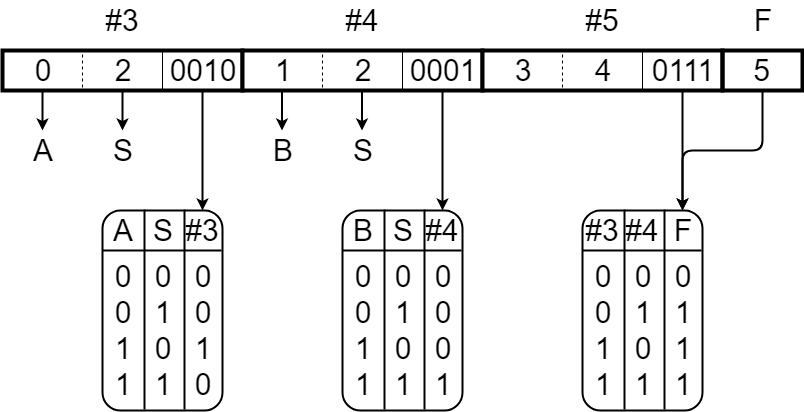
\includegraphics[width=0.7\textwidth]{img/genotype.png}
	\caption{Primjer genotipa rješenja za multiplekser}
	\label{fig:genotype}
\end{figure}

Naravno, navedeni genotip nije jedini mogući. Korištenje niza cijelih brojeva predstavlja kompromis između učinkovitosti i jednostavnosti. Intuitivnije jest korištenje strukture nalik stablu, gdje bi čvorovi sadržavali podatke o pojedinim CLB-ovima. Nedostatak jest veća računarska složenost jer se koristi više memorije. U cilju manje potrošnje memorije, moguće je koristiti niz bitova. Najveća ušteda ostvarila bi se za $m<5$. Na primjer, genotip na slici \ref{fig:genotype} koristi $10*32=320$ bitova memorije. Dovoljno je koristiti $3$ bita za ulaze ($M+n=3+3=6<2^{3}=8$) i $4$ bita za pregledne tablice. Rezultat bi bio $n*(m*3+4)+N*(3)=3*(2*3+4)+1*(3)=33$ bitova što donosi potrošnju od $33/320=10.3\%$. Razlika je velika, ali njena iskoristivost uvelike ovisi o programskom jeziku u kojem je genetski algoritam implementiran. Naime, programski jezik C podržava rad s pokazivačima (engl.\textit{pointer}) i bitovnim maskama (engl.\textit{bit mask}), dok programski jezik Java za niz bitova koristi nizove koji su duljine u višekratnicima broja $64$ (razred pod nazivom BitSet).

Izvedena je \textbf{paralelizacija genetskog algoritma} korištenjem skupa dretvi (engl.~\textit{thread pool}). Broj dretvi se odabire prije pokretanja algoritma. Na slici \ref{fig:threads} prikazan je dijagram koji prikazuje mehanizam usklađivanja skupa dretvi. Dretve čekaju u istovremenom redu čekanja (engl.~\textit{concurrent queue}). Genetski algoritam proslijedi populaciju u red čekanja, nakon čega se dretve "probude". Dretve paralelno izvode genetske operatore i pune novu populaciju. Koordinacija punjenja izvedena je korištenjem atomičkih operacija "usporedbe i zamjene" (engl.~\textit{compare and swap}, CAS). To su operacije koje su podržane na razini instrukcijskog seta procesora. CAS operacija garantira da će dretva pročitati trenutnu vrijednost varijable te da će istovremena promjena pročitane varijable biti odmah vidljiva svim ostalim dretvama. Prekid rada dretvi ostvaruje se na jedan od $2$ moguća načina. Normalan način zaustavljanja dretvi jest ubacivanje posebnih markera u red čekanja (engl.~\textit{red pill}). Dretva prepoznaje marker i prestaje s radom. Iznimno, omogućeno je zaustavljanje dretvi usred računanja sljedeće populacije.

\begin{figure}[htb]
	\centering
	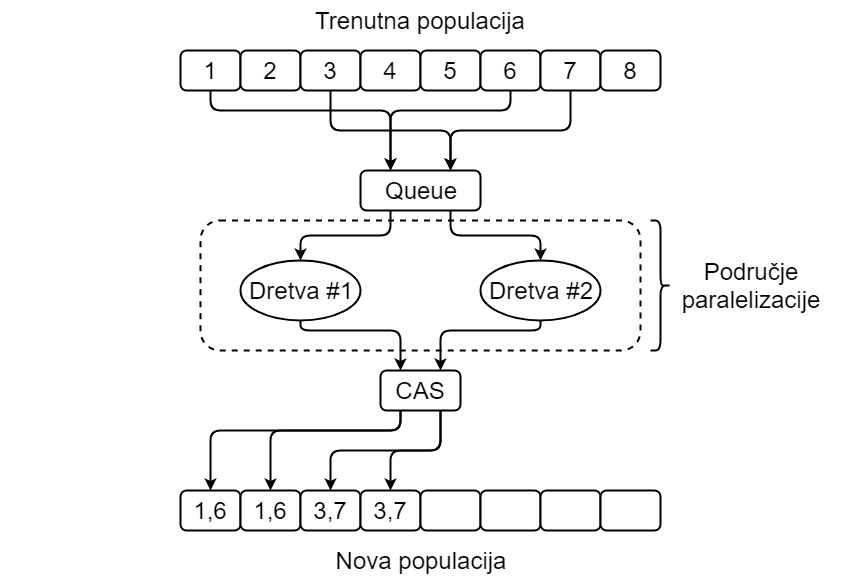
\includegraphics[width=0.8\textwidth]{img/threads.png}
	\caption{Usklađivanje rada dretvi pomoću reda čekanja i CAS operacija}
	\label{fig:threads}
\end{figure}

Za \textbf{ocjenjivanje kvalitete jedinke} koristi se najveći mogući broj poklapanja izlaza CLB-ova i Booleovih funkcija. Postupak evaluacije prolazi kroz sve kombinacije ulaznih varijabli te za trenutnu kombinaciju izračuna izlaz ($0$ ili $1$) svakog CLB-a i zapisuje ga u niz bitova duljine $n$. Zatim se u zasebno polje dimenzija $n*N$ povećava brojač za svako podudaranje izlaza CLB-a s nekom od Booleovih funkcija. Nakon prolaska kroz sve kombinacije, odabire se po jedan CLB s najviše podudaranja za svaku Booleovu funkciju. Zbroj podudaranja svih funkcija dijeli se s najvećim mogućim brojem podudaranja kako bi se dobila vrijednost u rasponu $[0, 1]$. Dobivena vrijednost uzima se kao kvaliteta (engl.~\textit{fitness}) jedinke. Izlaz CLB-a se sprema i ponovno koristi (engl.~caching), a računa se samo ako se promijenila vrijednost ulazne varijable o kojoj CLB ovisi. Omogućeno je gašenje ove funkcionalnosti za potrebe testiranja. Računanje ovisnosti o ulazima izvodi se na početku evaluacije, a rezultat je polje bitova dimenzija $M*n$. Ovime se postiže ubrzanje algoritma.

Za operator selekcije koristi se \textbf{turnirska selekcija} koja nasumično uzme $3$ jedinke iz populacije te odabire najbolju. Operator selekcije se ne mijenja pa nije parametar algoritma. Veličina turnira odabrana je prema prethodnom iskustvu i testiranju. Povećanje selekcijskog pritiska ne poboljšava performanse. Veličina elitizma je konfigurabilna, a pretpostavljena vrijednost jest $0.1\%$ veličine populacije s minimalnom vrijednošću $2$. Poželjan je malen elitizam kako bi se sačuvala raznolikost jedinki. Često je prisutno nekoliko najboljih jedinki u populaciji koje imaju jednaku kvalitetu pa ih se zato sačuva nekoliko, a ne samo jedna. Veličina elitizma ne sudjeluje u konačnoj optimizaciji algoritma. Za pohranu trenutne i nove populacije koriste se $2$ ista dijela memorije. Nova populacija nakon svake generacije postaje trenutnom populacijom, a memorija na kojoj se nalazila trenutna populacija koristi se za sljedeću novu populaciju. Ovime se uvelike ubrzava rad algoritma jer alokacija nove memorije i oslobađanje nekorištene memorije zahtijevaju puno vremena.

Koriste se $3$ vrste \textbf{operatora križanja}: jednostruko križanje, križanje s $2$ prekidne točke te "rekurzivno" križanje. Jednostruko križanje je zapravo jednako križanju s $2$ prekidne točke tako da je točno $1$ CLB između prekidnih točaka. Odabir prekidnih točaka je nasumičan. Prvo se nasumično odabere duljina intervala križanja u rasponu $[1, n-1]$, a zatim se nasumično odabere položaj intervala. Prva prekidna točka je početak intervala, a druga prekidna točka je kraj intervala. Obje vrste križanja koriste se u $2$ inačice: poravnate i "pomaknute". Poravnata inačica samo zamijeni blokove na istim pozicijama. "Pomaknuta" inačica koristi zasebne intervale za svakog roditelja. Pri zamjeni blokova preračunavaju se indeksi ulaza kako bi se očuvala povezanost blokova unutar intervala. Veze koju se ne mogu popraviti postave se na nasumične vrijednosti. "Rekurzivno" križanje nasumično zamijeni jedan CLB i sve CLB-ove koji su potrebni za izračun njegovog izlaza. Drugim riječima, zamijene se svi CLB-ovi koji su ispod njega u stablu ovisnosti. "Rekurzivno" križanje je uvijek poravnato zbog jednostavnosti.

Koristi se $5$ vrsti \textbf{operatora mutacija} podijeljenih u dvije kategorije: $2$ vrste mutacija ulaza te $3$ vrste mutacija pregledne tablice. Potpuna mutacija ulaza postavi sve ulaze CLB-a na nasumične vrijednosti. Nepotpuna mutacija ulaza promijeni određen broj ulaza, ovisno o vjerojatnosti mutacije. Analogno tome, potpuna mutacija pregledne tablice mijenja sve bitove u tablici, dok višestruka mijenja određen broj. Zadnja vrsta mutacije jest mutacija koja nasumično odabere $2$ CLB-a te kopira tablicu iz prvog u drugi. Kopiranje pregledne tablice pokazalo se kao učinkovit operator mutacije kada optimalno rješenje treba sadržavati veći broj jednakih tablica.

Algoritam koristi niz \textbf{kriterija zaustavljanja} koji su navedeni po redu provjeravanja. Prvi jest prag kvalitete. U slučaju da genetski algoritam uspije pronaći ispravno rješenje, odmah se zaustavlja i vraća pronađeno rješenje rješavaču. Drugi kriterij jest maksimalan broj generacija. Ovaj kriterij nije apsolutan tj.~algoritam neće stati u slučaju da se najbolje rješenje unaprijedilo u određenom broju prošlih generacija (parametar). Treći kriterij jest stagnacija najboljeg rješenja. Algoritam se zaustavlja ako određen broj uzastopnih generacija (parametar) ne uspije povećati kvalitetu najboljeg rješenja. Četvrti i zadnji kriterij jest vremensko ograničenje izvođenja. Vrijeme se zadaje u milisekundama i provjerava se na kraju svake generacije. Još jedan mogući način zaustavljanja jest samostalno gašenje dretvi. Naime, genetski algoritam čeka da dretve popune novu populaciju. Ako su dretve završile, a nova populacija nije popunjena, genetski algoritam završava s izvođenjem.

Ugrađen je jednostavan \textbf{mehanizam simuliranog kaljenja} u modificirani genetski algoritam. Postotak preostalog broja generacija koristi se kao parametar temperature $T$ kod simuliranog kaljenja. Početna temperatura $T_{0}$ jest $1.0$, a konačna temperatura $T_{f}$ jest parametar algoritma koji se ovdje naziva "prag kaljenja" (oko $0.2$). Umjesto funkcije prihvaćanja $P(\Delta f, T)$ koristi se pravilo prihvaćanja poboljšavajućeg rješenja. Nakon svake selekcije roditelja odredi se hoće li se prihvaćati samo djeca s većom kvalitetom. Nasumično se uzme vrijednost iz intervala $t=[T_{f}, T_{0}]$ i ako je $t<T$ onda se rezultati križanja i mutacije prihvaćaju samo ako su kvalitetniji. Mutacija jako rijetko unaprijedi rješenje pa se ne izvodi ako je dijete kvalitetnije od oba roditelja. Vjerojatnost prihvaćanja lošijih rješenja linearno opada kako se temperatura $T$ približava pragu kaljenja $T_{f}$. Temperatura se ujedno koristi kao vjerojatnost mutacije. Na primjer, višestruka mutacija pregledne tablice koristi temperaturu $T$ kao parametar standardne devijacije normalne razdiobe. Broj mutiranih bitova jednak je $\lvert g(\mu, \sigma) \rvert = \lvert g(1, \frac{lT}{3}) \rvert$ gdje je $g$ funkcija normalne razdiobe, a $l$ je broj bitova u preglednoj tablici. Nakon što temperatura prijeđe prag kaljenja, algoritam prestaje izvoditi križanje te se oslanja na precizne mutacije. Ovo degradira genetski algoritam u lokalno pretraživanje. Svrha lokalnog pretraživanja jest nadomjestiti neučinkovitost genetskog algoritma pri pronalasku rješenja u lokalnom optimumu.

Zadnji mehanizam odnosi se na minimalan broj uzastopnih stagnirajućih generacija (nisu poboljšale najbolje rješenje) potrebnih za poštivanje maksimalnog broja generacija. GA ne prekida rad sve dok se najbolje rješenje dovoljno često unapređuje. Ipak, sigurno je da će GA završiti u konačnom broju generacije jer je funkcija kvalitete diskretna (broj preklapanja izlaza blokova i funkcija).

\subsection{Implementirana heuristika} \label{subsec:solver}

Modificirani genetski algoritam iz prethodnog odjeljka koristi se kao podprogram u sklopu glavnog programa koji će se ovdje nazivati "rješavač". Zajedno oni čine konačnu implementaciju heuristike. Zadaća rješavača jest \textbf{procijeniti najmanji potreban broj CLB-ova} za ostvarenje zadanog Booleovog vektora. Postoje $3$ postupno složenija načina procjene. Osnovna procjena zasniva se na rješavanju korištenjem "grube sile" (engl.~\textit{brute force}). Ovaj postupak garantira pronalazak rješenja u vrlo kratkom vremenu. Dobiveno rješenje najčešće je loše kvalitete (velik broj CLB-ova), ali katkad je prihvatljivo. Ideja postupka jest stvaranje "\textbf{multipleksorskog stabla}" kao što je prikazano na slici \ref{fig:brute}. Stablo se sastoji od $7$ CLB-ova. Skroz desni CLB predstavlja korijen stabla i njegov izlaz jednak je Booleovoj funkciji $F$. Gornji ulaz ($A$ za korijenski CLB) jest adresni ulaz, a preostala $2$ ulaza su podatkovni. Funkcionalnost multipleksera postiže se posebno konstruiranom preglednom tablicom s vrijednostima $00110101$. Ako je $A=0$ onda se koristi prva polovica tablice. Nadalje, ako je drugi ulaz (izlaz iz CLB-a $\#9$) jednak $0$ onda je izlaz $0$ bez obzira na treći ulaz. Slično je i za ostale kombinacije ulaza. CLB-ovi $\#9$ i $\#10$ rade po istom principu. Do razlike dolazi u listovima stabla tj.~u krajnjim čvorovima stabla. Pregledne tablice CLB-ova $\#5-\#8$ redom sadrže dijelove tablice istinitosti Booleove funkcije $F$. Tablica istinitosti očita se od gore prema dolje. Pregledne tablice označene žutom bojom sadrže jednake vrijednosti. Kako CLB-ovi $\#7$ i $\#8$ imaju i iste ulaze, njihovi izlazi su jednaki za sve kombinacije ulaza. Algoritam, nakon izgradnje stabla, simulira sve kombinacije ulaza te prepoznaje CLB-ove s jednakim izlazima. Nepotrebni CLB-ovi se uklanjaju kao što je prikazano iscrtkanim linijama. CLB-ovi $\#8$ i $\#10$ prestaju biti dio rješenja. Naravno, tablica istinitosti namjerno je odabrana tako da se ponavljanju nizovi $01001001$ na kraju.

\begin{figure}[htb]
	\centering
	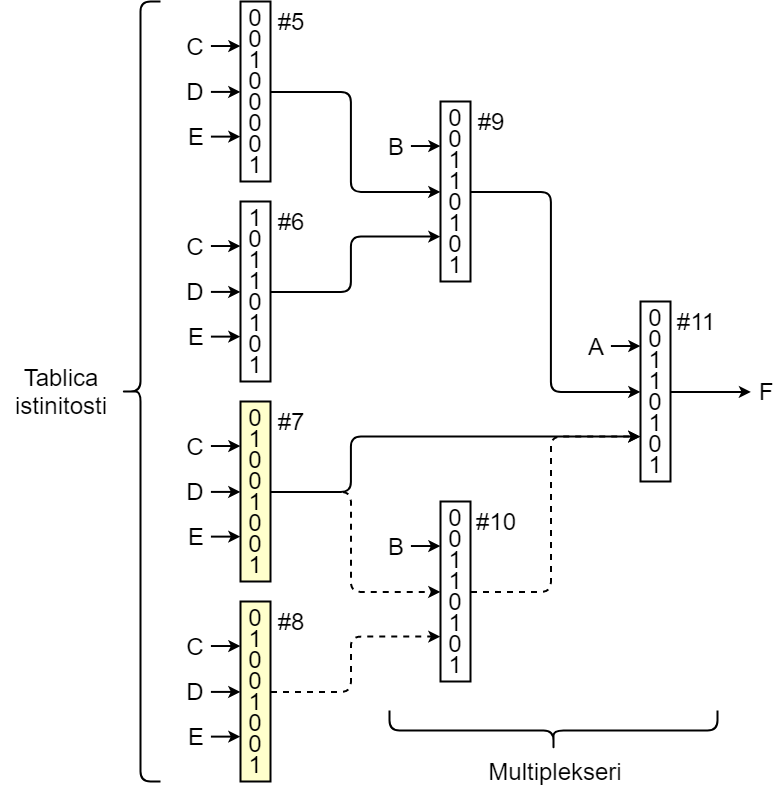
\includegraphics[width=0.7\textwidth]{img/brute.png}
	\caption{Korištenje CLB-ova u izgradnji "multipleksorskog stabla"}
	\label{fig:brute}
\end{figure}

Konstrukcija pregledne tablice i struktura multipleksorskog stabla ovise o broju ulaza u CLB $m$ i veličini tablice istinitosti Booleove funkcije. Algoritam podržava sve moguće kombinacije unutar razumnih ograničenja tj.~nije dozvoljeno stvaranje prevelikih stabala (više tisuća CLB-ova). Za $m=4$ i $m=5$ višak ulaza se zanemaruje. Ako je $m \geq 6$ onda se konstruiraju multiplekseri s $2$ adresna ulaza (i $4$ podatkovna ulaza). Algoritam je isti, jedino se izračun mijenja. Pregledna tablica multipleksorskog CLB-a sadrži $64$ bitova što je previše za prikaz kao na slici \ref{fig:brute} pa je zato dana u nastavku kao $00000000111111110000111100001111 \allowbreak 00110011001100110101010101010101$. Jedini poseban slučaj jest kada je broj ulaza CLB-a jednak $m=2$. Tada je potrebno koristiti $3$ $2$-ulazna CLB-a za ostvarenje multipleksera jer pripadni Booleov izraz $Y_{2/1} = (A \cdot \overline{S}) + (B \cdot S)$ sadrži $3$ binarne operacije. Još je potrebno koristiti $M-m=M-2$ CLB-ova za negaciju adresnih ulaza. Na slici \ref{fig:full-adder-s} prikazano je rješenje izlaza $S$ potpunog binarnog zbrajala korištenjem $2$-ulaznih CLB-ova. Označena su $3$ bloka koja zajedno tvore $3$-ulazni multiplekser. CLB $\#7$ na prvi ulaz prima adresni ulaz $A$, dok CLB $\#6$ na prvi ulaz prima negiranu vrijednost adresnog ulaza $A$. Negiranje ulaza $A$ izvodi se pomoću CLB-a s indeksom $\#3$. CLB-ovi $\#4$ i $\#5$ sadrže tablicu istinitosti izlazne funkcije $S$. Ovakvo rješenje troši $3$ puta više blokova od rješenja koje koristi $3$-ulazne CLB-ove te se još troši $M-m$ blokova za negacije ulaza koji se koriste kao adrese za multipleksiranje.

\begin{figure}[htb]
	\centering
	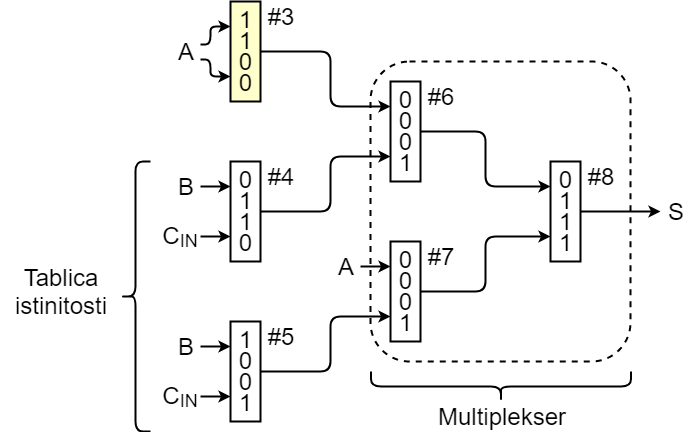
\includegraphics[width=0.6\textwidth]{img/full_adder_s.png}
	\caption{Rješenje funkcije $S$ potpunog zbrajala pomoću $2$-ulaznih CLB-ova}
	\label{fig:full-adder-s}
\end{figure}

Drugi postupak rješavanja uključuje korištenje modificiranog genetskog algoritma kako bi se našla \textbf{pojedinačna rješenja} za svaku Booleovu funkciju. Postupno se poboljšava procjena broja blokova potrebnih za optimalno rješenje. Broj blokova u stablu iz prethodnog postupka određuje \textbf{gornju granicu} procjene (oznaka $n_{max}$), dok je \textbf{donja granica} na početku jednaka $n_{min}=1$. Početna procjena $n_{procjena}=\frac{M}{m}$ jednaka je omjeru broja ulaza Booleove funkcije te broja ulaza u pojedinog CLB-a. Zatim genetski algoritam pokušava naći ispravno rješenje za trenutnu procjenu broja blokova. Neuspjeh pronalaska rješenja smatra se apsolutnim tj.~heuristika pretpostavlja da ne postoji konfiguracija zadanog broja blokova takva da implementira željenu Booleovu funkciju. Isto vrijedi i za manje brojeve blokova pa se trenutna procjena uzima kao donja granica (oznaka $n_{min}=n_{procjena}$). Jedino što preostaje jest povećanje procjene. Linearno povećanje procjene bilo bi najjednostavnije, ali potrebno je uzeti u obzir vrijeme izvođenja algoritma. Udvostručavanje procjene broja blokova ubrzava pronalazak rješenja u većini slučajeva. Udvostručavanje procjene slično je binarnoj pretrazi koja prepolavlja gornju granicu. Razlog zašto se počinje s malenom početnom procjenom jest vrijeme izvođenje genetskog algoritma. Naime, brže je pokretati GA na više manjih procjena, nego odmah početi sa sredinom intervala ($\frac{n_{max}}{2}$) kao što to radi binarno pretraživanje. U slučaju da GA pronađe rješenje, trenutna procjena postaje gornjom granicom $n_{max}=n_{procjena}$. Prisutnost rješenja mijenja određivanje trenutne procjene u binarno pretraživanje između gornje $n_{max}$ i donje granice $n_{min}$. Neuspjeh genetskog algoritma podiže donju granicu, dok pronalazak novog (najboljeg) rješenja spušta gornju granicu. Postupak prestaje čim se poklope gornja i donja granica. Ako se udvostručavanjem početne procjene prijeđe preko gornje granice onda se procjena postavlja na $n_{procjena}=n_{max}-1$. Nemogućnost pronalaska rješenja s tom procjenom zaustavlja pretragu, a za rješenje trenutne Booleove funkcije uzima se pripadno stablo dobiveno postupkom "grube sile". Opisani postupak ponavlja se za svaku Booleovu funkciju, a konačno rješenje dobije se spajanjem rješenja pojedinačnih funkcija. Postoji mogućnost da rješenja sadrže jednake blokove koje algoritam spajanja prepoznaje i uklanja iz konačnog rješenja.

Treći postupak rješavanja sličan je prethodnom, ali uz sljedeće razlike. Genetski algoritam rješava \textbf{sve funkcije odjednom}. Gornja granica postavlja se na broj CLB-ova u konačnom rješenju iz prethodnog postupka. Početna procjena jednaka je prosjeku broja blokova uspješno riješenih Booleovih funkcija iz prethodnog postupka. Početna procjena je $n_{procjena}=2$ ako niti jedna funkcija nije riješena. Ako se ne pronađe rješenje onda se uzima rješenje iz prethodnog postupka što može biti i stablo iz prvog postupka. Razlog tome jest što postoji mogućnost odabira načina rješavanja cjelokupnog programa. "Grub" način rada koristi samo prvi postupak, jako je brz i kao rezultat vraća multipleksorsko stablo. "Brz" način rada koristi vremensko ograničenje za drugi i treći postupak (otprilike $10$ sekundi po funkciji). "Normalan" način rada koristi vremensko ograničenje samo u zadnjem postupku (otprilike minuta po funkciji). "Potpun" način rada ne koristi vremenska ograničenja. Prekoračenje vremenskog ograničenja zaustavlja izvođenje postupka te se uzima trenutno najbolje rješenje (ako ono postoji). 

U svrhu optimizacije genetskih operatora ugrađen je mehanizam praćenja "\textbf{statistike operatora}". Praćenje statistike usporava algoritam pa nije preporučeno ako nije potrebno. Razlog usporavanja proizlazi iz potrebe za dvostrukom evaluacijom djece u genetskom algoritmu. Pamti se kvaliteta jedinke prije svakog korištenja genetskog operatora. Zatim se uspoređuje s dobivenom jedinkom te se ažurira statistika za taj operator ovisno o razlici kvalitete. To znači da se evaluacija radi i nakon križanja i nakon mutacije (inače se radi samo nakon zadnjeg operatora). Prate se $4$ vrijednosti za svaku vrstu operatora: broj korištenja, broj pogoršanja jedinke, broj poboljšanja jedinke te broj puta koliko je operator uspio poboljšati najbolje rješenje u generaciji. Statistika se akumulira te se ispisuje na kraju algoritma.

Na kraju je potrebno spomenuti $5$ dodatnih parametara koji se koriste u drugom i trećem postupku (ne koriste pri izgradnji stabla). Prvi parametar jest \textbf{maksimalan broj pokušaja} tj. broj pokretanja GA u slučaju da GA ne uspije način rješenje isprve. Naime, GA često ovisi o kvaliteti početne populacije te se može dogoditi da ne uspije naći rješenje u prvom pokušaju. Kako se ipak ne bi trošilo previše vremena s nerješivim brojem CLB-ova (procjena je premalena), koristi se još $3$ dodatna parametra. Prvi od njih jest maksimalan broj uzastopnih pokušaja koji su rezultirali s rješenjem ispod određenog praga. Prag poprima jednu od $2$ moguće vrijednosti ovisno o tome je li GA dosad našao ispravno rješenje. Ako rješenje postoji onda je pretpostavljena vrijednost praga je $prag_{1}=0.97$, a inače iznosi $prag_{2}=0.93$.

%%%%%
%%%%%
%%%%%

\section{Grafičko sučelje} \label{sec:gui}

Kako bi se razvijeni algoritam mogao lakše koristiti, napravljeno je grafičko sučelje (engl.~\textit{graphical user interface}, GUI) korištenjem Swing-a. Sučelje podržava lokalizaciju i nudi izbor između $2$ jezika: \textbf{engleski i hrvatski}. Na slici \ref{fig:gui} može se vidjeti izgled glavnog prozora GUI-a. Veličina prozora je promjenjiva uz automatsko skaliranje većine komponenti. Na vrhu okvira prozora (engl.~\textit{frame}) jest datotečni put (engl.~\textit{file path}) trenutne datoteke nakon kojeg slijedi naziv aplikacije JFPGA. Odmah ispod nalazi se izbornik s alatima (engl.~\textit{menu}) u kojem se može pristupiti svim funkcionalnostima sučelja. Ispod izbornika nalazi se prostor s karticama (engl.~\textit{tab}). Svaka kartica sadrži ime datoteke trenutne sjednice (engl.~\textit{session}), ikonu spremljenosti podataka te gumb za zatvaranje sjednice. Sjednice omogućuju istovremeno korištenje različitih skupova podataka uz korištenje samo jednog prozora. Ova mogućnost jest opcionalna i u većini slučajeva dovoljno je koristiti $1$ sjednicu. Sučelje sjednice okvirno je podijeljeno u $5$ stupaca. Prvi stupac koristi se za unos i prikaz Booleovih funkcija. Drugi stupac sadrži popis Booleovih funkcija (i popratne alate). Treći stupac sadrži popis Booleovih vektora i popratne alate. Četvrti stupac koristi se za unos parametara i pokretanje algoritma. Peti i zadnji stupac sadrži generirana rješenja. Osnovan opis komponenti dan je u odjeljku \ref{subsec:osnove_koristenja}, dok se detaljan opis svih komponenti nalazi u odjeljku \ref{subsec:dodatne_mogucnosti}.

\begin{figure}[htb]
	\centering
	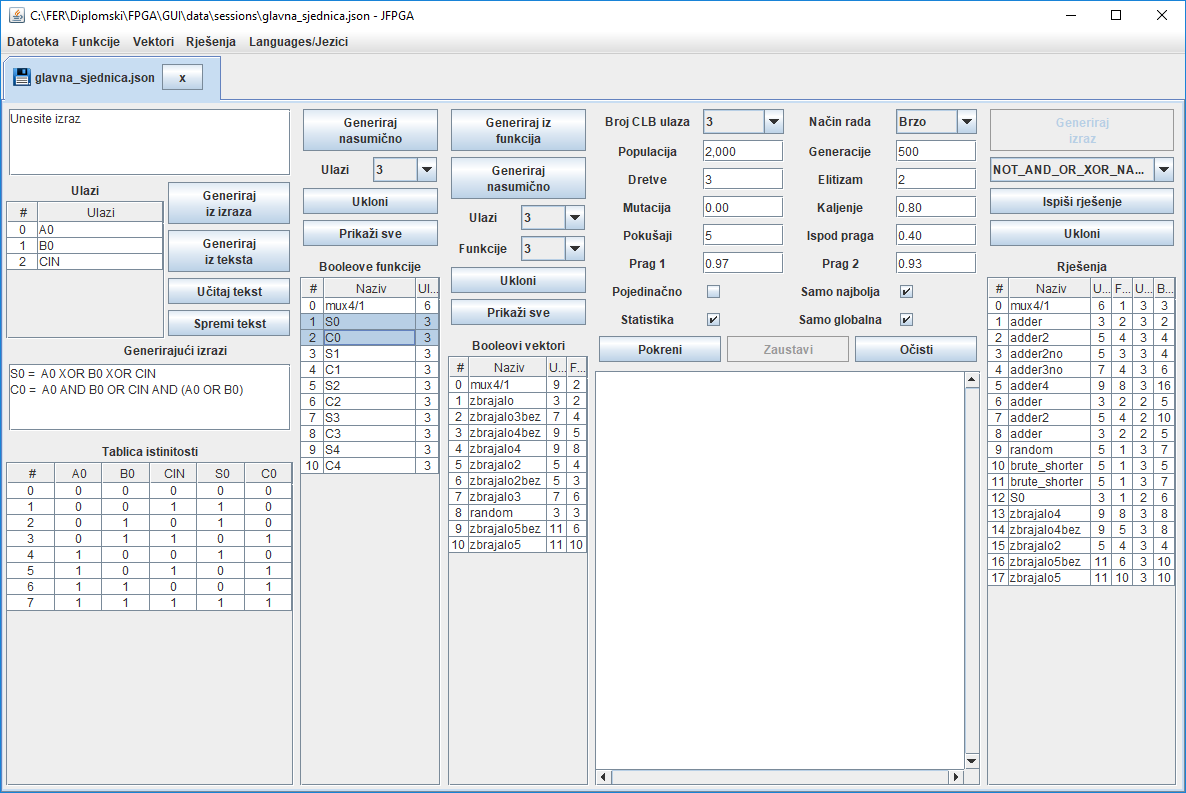
\includegraphics[width=1.0\textwidth]{img/GUI.png}
	\caption{Prikaz glavnog prozora grafičkog sučelja}
	\label{fig:gui}
\end{figure}

\subsection{Osnove korištenja} \label{subsec:osnove_koristenja}

Za početak je potrebno postaviti jezik sučelja. Izbornik "Languages/Jezici" nudi izbor između engleskog jezika i hrvatskog jezika. Ovdje će se koristiti hrvatski jezik. Sljedeći korak jest stvoriti \textbf{novu sjednicu} ili otvoriti postojeću što u izborniku "Datoteka" odgovara opcijama "Nova" i "Otvori". Stvorit će se nova kartica odmah ispod izbornika s početnim nazivom "Nova sjednica" ili s nazivom pripadne datoteke (ako se otvori postojeća sjednica). Unos Booleovih funkcija moguće je ostvariti na $4$ različita načina. Najjednostavniji način unosa Booleove funkcije jest pomoću Booleovog izraza. U gornjem kutu skroz lijevog stupca nalazi se \textbf{područje za unos teksta} koje sadrži početni tekst "Unesite izraz". Ispod područja za unos nalazi se gumb s nazivom "Generiraj iz izraza" koji pokreće pretvorbu unesenog izraza u funkciju. Na primjer, unosom teksta "f1 = a and (b or c)" stvorit će se funkcija s nazivom "f1" koja odgovara Booleovom izrazu $a \cdot (b + c)$. Znak jednakosti "=" može se izostaviti, a u tom slučaju funkcija poprima pretpostavljenu vrijednost.

Popis funkcija nalazi se u listi na kraju drugog stupca ispod teksta "Booleove funkcije". Svaki redak liste sadrži jednu Booleovu funkciju s prikazom sljedećih osnovnih informacija: redni broj u listi (zaglavlje "\#"), ime funkcije (zaglavlje "Naziv") te broj ulaza funkcije (zaglavlje "Ulazi", skraćeno "U"). Moguće je klikom označiti jednu ili više funkcija. Odabir više redaka u listi izvršava se pomoću uobičajenih tipki na tipkovnici: "Shift" za neprekinuti interval te "Ctrl" za dodavanje pojedinačnih redaka. Trenutno odabrani retci označeni su tamnijom bojom. Dvostrukim klikom na naziv funkcije omogućena je \textbf{promjena naziva}.

Prikaz podataka odabranih funkcija nalazi se u prvom stupcu. Na kraju prvog stupca nalazi se \textbf{tablica istinitosti}. Vrijednosti u tablici istinitosti mogu se mijenjati (dvostruki klik) ako je odabrana samo $1$ Booleova funkcija. Odmah iznad tablice istinitosti ispod teksta "Generirajući izrazi" nalazi se \textbf{popis Booleovih izraza} iz kojih su odabrane funkcije generirane. Još iznad, lijevo od gumba za unos, nalazi se \textbf{popis ulaznih varijabli} za odabrane funkcije. Duplikati se ne prikazuju kod više odabranih funkcija. Ulazi se mogu preimenovati (dvostruki klik) čak i kada je odabrano više funkcija.

Za korištenje algoritma potrebno je stvoriti Booleov vektor iz odabranih funkcija čak i ako se želi riješiti samo $1$ Booleova funkcija. Vektor se stvori pomoću gumba s nazivom "Generiraj iz funkcija" koji se nalazi na vrhu trećeg stupca. Popis Boolevih vektora nalazi se na kraju trećeg stupca u listi koja je slična listi Booleovih funkcija. Pritom treća vrijednost u retku prikazuje ukupan broj ulaza u Booleov vektor, dok četvrta vrijednost prikazuje broj Boolevih funkcija iz kojih je vektor generiran. Ulazi s istim nazivima smatraju se istim pa broj ulaza u vektor može biti manji nego zbroj ulaza pojedinih Booleovih funkcija. Odabir i preimenovanje rade na isti način kao i kod liste funkcija.

Četvrti stupac sastoji se od $2$ dijela. Gornji dio sastoji se od raznih komponenti koje služe za unos parametara algoritma. Najvažniji parametar nalazi se na početku i to desno od teksta "Broj CLB ulaza". Klikom na njega otvara se popis dozvoljenih vrijednosti za broj ulaza u pojedini konfigurabilni logički blok (CLB). Donji dio četvrtog stupca sastoji se područja za tekstualni ispis te pripadnih gumba koji se nalaze odmah iznad njega. Prvi gumb \textbf{pokreće izvršavanje} algoritma, dok drugi gumb \textbf{zaustavlja izvođenje}. Treći gumb s nazivom "Očisti" služi za \textbf{brisanje izlaznog teksta}. 

Zadnji stupac sučelja sadrži popis svih rješenja koja su dosad generirana. Rješenja su smještena u listi na sličan način kao i Booleove funkcije (i vektori). Početni naziv rješenja jednak je nazivu Booleovog vektora iz kojeg je nastao. Svaki redak, osim indeksa i naziva rješenja, sadrži sljedeće $4$ vrijednosti: broj ulaza i broj funkcija u vektoru, broj ulaza pojedinog CLB-a te broj CLB-ova u rješenju. \textbf{Ispis rješenja} moguć je klikom na gumb s nazivom "Ispiši rješenje". Preporuča se brisanje izlaznog teksta (gumb "Očisti") prije ispisivanja rješenja kako bi ispis bio čitljiviji. Sadržaj ispisa rješenja podijeljen je u $3$ dijela. Prvi dio ispisa sadrži tekstualnu reprezentaciju podataka koja nije zanimljiva običnom korisniku, ali je korisna za provjeru podataka. Drugi dio ispisa sadrži tablicu istinitosti za sve CLB-ove i sve Booleove funkcije u rješenju. Tablica je korisna za provjeru valjanosti izlaza CLB-ova.

Treći dio ispisa sadrži \textbf{tekstualni oblik konfiguracije blokova}. Na slici \ref{fig:solution-text} prikazan je tekstualni oblik rješenja dobivenog za $2$-bitno potpuno binarno zbrajalo. Rješenje se sastoji od ukupno $13$ redaka: $5$ redaka za ulazne blokove, $4$ redaka za CLB-ove te $4$ redaka za Booleove funkcije. Svaki redak za ulazni blok sastoji se od $3$ dijela: vektor binarnih vrijednosti korištenja, indeks bloka te naziv ulazne varijable. Ulazni blokovi su sortirani po  abecednom redosljedu. Vektor korištenja ima $N$ binarnih vrijednosti, jednu za svaku Booleovu funkciju. Vrijednost na indeksu $i$ jednaka je $1$ ako $i$-ta funkcija koristi tu ulaznu varijablu. Retci s CLB-ovima isto sadrže vektor korištenja gdje je vrijednost na indeksu $i$ jednaka $1$ ako $i$-ta funkcija koristi taj CLB. Pritom se podrazumijeva da funkcija koristi sve CLB-ove u podstablu. Na primjer, funkcija $S_{1}$ na slici \ref{fig:solution-text} kao izlaz koristi CLB s indeksom $8$. Indeks funkcije $S_{1}$ je $i=2$ ($0$-indeksirano) pa zato vektor korištenja CLB s indeksom $8$ ima vrijednost $1$ na poziciji $i=2$. Nakon vektora korištenja slijedi indeks bloka te zatim parametri CLB-a. Prvih $m=3$ brojeva predstavlja ulaze koji pokazuju na indekse blokova. Ostatak retka sadrži binarni prikaz pregledne tablice (LUT). U nastavku slijedi primjer jednostavne simulacije prvog CLB-a (indeks $5$). Neka je ulazna kombinacija jednaka $10001$ tj.~vrijednosti ulaza jednake su $A_{0}=1$, $A_{1}=0$, $B_{0}=0$, $B_{1}=0$ i $C_{IN}=1$. Ulazi u blok $\{4, 2, 0\}$ odgovaraju ulaznim blokovima s varijablama $\{C_{IN}=1, B_{0}=0, A_{0}=1\}$. Ulazne vrijednosti tvore binarni prikaz broja $101_{2}=5_{10}$ pa je izlaz CLB-a jednak petoj vrijednosti u preglednoj tablici ($0$-indeksirano čitano s lijeva) što je jednako $1$.

\begin{figure}[htb]
	\centering
	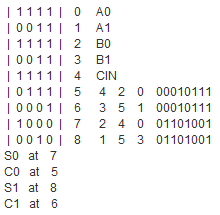
\includegraphics[width=0.33\textwidth]{img/solution_text.png}
	\caption{Rješenje za $2$-bitno potpuno zbrajalo u tekstualnom obliku}
	\label{fig:solution-text}
\end{figure}

\subsection{Dodatne mogućnosti} \label{subsec:dodatne_mogucnosti}

Grafičko sučelje sadrži mnoštvo dodatnih mogućnosti koje nisu spomenute u odjeljku \ref{subsec:osnove_koristenja}. Većina ih se odnosi na unos, pohranu i mijenjanje $3$ vrsti podataka: funkcija, vektora i rješenja. Kao format spremanja podataka koriste se tekstualni format s ekstenzijom ".txt" te JSON format s ekstenzijom ".json". JSON format služi za spremanje Java objekata i koristi se kao zamjena za serijalizaciju. Razlog tome jest što je JSON format univerzalan i napravljen da bude čitljiv ljudskom oku. Spremanje i unos podataka pomoću JSON datoteka može se koristiti za integraciju s ostalim programima kao što je program za testiranje u poglavlju \ref{chapter:results}.

Sjednica se označi kao promijenjena ako se dogodi promjena u podacima. To je vidljivo po promjeni boje ikone u kartici (lijevo od naziva sjednice). U slučaju da se pokuša zatvoriti sjednica koja sadrži izmjene, prikaže se \textbf{dijalog za potvrdu}, a po potrebi i dijalog za spremanje. Spremanjem sjednice pohranjuju se sve Booleove funkcije i vektori te sva rješenja. U slučaju korištenja više sjednica, onemogućeno je pokretanje algoritma ako se on već izvodi u nekoj od sjednica.

Sve $3$ liste s podacima (funkcije, vektori i rješenja) podržavaju sljedeće funkcionalnosti: \textbf{uklanjanje}, \textbf{poništavanje uklanjanja}, \textbf{spremanje} te \textbf{učitavanje}. Sve se izvršavaju se na odabranim elementima, osim poništavanja elemenata (engl.~\textit{undo}) koja pamti povijest uklanjanja te ponovno vraća izbrisana elemente. Dodatno, liste s Booleovim funkcijama i vektorima podržavaju \textbf{dupliciranje} elemenata te prikazivanje svih dostupnih elemenata. Naime, moguće je \textbf{privremeno prikazivanje} samo onih elemenata koji su dio roditeljskog elementa. Konkretno, dvostrukim klikom na broj funkcija u listi Booleovih vektora promijenit će se sadržaj liste s Booleovim funkcijama. Ona će privremeno prikazivati funkcije iz kojih je vektor generiran. Ova funkcionalnost je korisna kada se žele vidjeti detalji funkcija u vektoru, a ujedno se te funkcije mogu i promijeniti. Ovakav prikaz je privremen te se prekida promjenom odabira vektora ili pomoću gumba s nazivom "Prikaži sve". Slično je moguće i s rješenjima. Dvostrukim klikom na broj funkcija u listi s rješenjima prikazat će se vektor iz kojeg je rješenje generirano. Jedina razlika jest što se vektor ne može promijeniti zbog očuvanja valjanosti rješenja.

U odjeljku \ref{subsec:osnove_koristenja} spomenut je samo osnovni način unosa Booleove funkcije pomoću Booleovog izraza. Još je podržano tzv.~\textbf{simboličko povezivanje} Booleovih funkcija tj.~funkcije mogu koristiti ostale funkcije kao ulaz. Simboličko povezivanje je veoma korisno kod unosa funkcija kao što su izlazne funkcije višebitnih potpunih zbrajala. Funkcije koje se koriste kao ulaz ne moraju biti odabrane prilikom stvaranja Booleovog vektora. U tom slučaju provjeravaju se sve raspoložive funkcije. Zadnji način unosa Booleovih funkcija jest \textbf{upisivanjem tablice istinitosti} u područje za unos teksta te pritiskom na gumb s nazivom "Generiraj iz teksta". Moguće je unijeti nazive ulaznih varijabli prije same tablice, ali to nije potrebno ako su pretpostavljene vrijednosti ("a", "b", "c", itd.) prihvatljive. Na primjer, unosom teksta "f1 = a b c 00000111" stvorit će se isti Booleova funkcija kao i u odjeljku \ref{subsec:osnove_koristenja} ("f1 = a and (b or c)"). Kao i prije, definiranje naziva funkcije prije znaka jednakosti "=" je opcionalno.

Omogućeno je i \textbf{nasumično generiranje} funkcija i vektora pomoću gumba s nazivima "Generiraj nasumično". Pritom se koriste padajući izbornici (engl.~\textit{combo box}) koji se nalaze ispod pripadnih gumba. Generiranje nasumične funkcije zahtijeva broj ulaza, dok generiranje nasumičnog vektora zahtijeva broj ulaza svake funkcije te broj funkcija. Kroz izbornik "Vektori" dostupan je još jedan način generiranja Booleovog vektora. Omogućeno je \textbf{generiranje rješivog vektora}. Klikom na opciju "Generiraj rješiv" prikaže se dijalog za unos broja CLB-ova. Klikom na "OK" stvori se vektor koji je sigurno rješiv sa zadanim brojem CLB-ova. Ostali parametri vektora te broj ulaza CLB-ova uzimaju se iz sučelja.

Gornji dio četvrtog stupca sadrži različite parametre algoritma. Osim broja ulaza CLB-ova, mogu se mijenjati sljedeći parametri algoritma za rješavanje: način rada, veličina populacije, broj generacija, broj dretvi, veličina elitizma, vjerojatnost mutacije te  prag kaljenja. Dodatno, mogu se mijenjati i sljedeći parametri rješavača: broj pokušaja, broj pokušaja ispod pragova, prvi i drugi prag, pojedinačno rješavanje, ispisivanje samo najboljih rješenja, korištenje statistike operatora te ispisivanje samo globalne statistike. Svi brojčani ulazi su ograničeni te se unos nedozvoljenih vrijednosti poništava. Dodatna funkcionalnost algoritma jest spremanje trenutnog rješenja u slučaju da se izvođenje algoritma prekine pomoću gumba s nazivom %TODO

Zadnja funkcionalnost odnosi se na rješenja koja su ostvarena pomoću $2$-ulaznih CLB-ova. U tom slučaju moguć je \textbf{ispis Booleovog izraza iz rješenja}. Odabirom prikladnog rješenje omogućava se korištenje gumba s nazivom "Generiraj izraz" koji se nalazi na vrhu petog stupca. Postupak generiranja izraza rekurzivno prolazi kroz CLB-ove i mapiranjem prevodi pregledne tablice u $16$ osnovnih Booleovih izraza s $2$ varijable. Pritom se mogu zadati $3$ različita mapiranja koja su dostupna u padajućem izborniku odmah ispod gumba "Generiraj izraz". Osnovno mapiranje ("NOT\_AND\_OR) koristi samo osnovne operatore. Naprednije mapiranje ("NOT\_AND\_OR\_XOR") uključuje i operator XOR. Pretpostavljeno mapiranje koristi svih $16$ operatora. Ova funkcionalnost proširena je i na tekstualni ispis rješenja čiji CLB-ovi imaju $2$ ulaza. Dodaje se ispis pripadnog Booleovog izraza nakon ispisa pregledne tablice svakog CLB-a.

%%%%%
%%%%%
%%%%%

\chapter{Rezultati} \label{chapter:results}

U ovom poglavlju nalaze se rezultati testiranja implementirane heuristike. Korišteni su jednaki računalni resursi za sva testiranja. Konkretno, korišteno je računalo s procesorom Intel i5-6600K ($4$ jezgre s taktom od $3.5$GHz) i radnom memorijom (RAM) s taktom od $2400$Mhz. Korištene su $3$ jezgre procesora kako bi se smanjio utjecaj izvođenja programa u pozadini operacijskog sustava.

%%%%%
%%%%%
%%%%%

\section{Optimizacija parametara}

U poglavlju \ref{chapter:impl} navedeni su svi parametri algoritma. Za učinkovit rad i dobre rezultate potrebno je optimizirati sve parametre. Optimizaciju je potrebno izvesti u nekoliko koraka zbog velikog broja parametara. Prvi korak jest optimizacija $3$ najvažnijih parametara: veličina populacije, broj generacija te broj pokušaja. Korišten je postupak pretrage po rešetci (engl.~\textit{grid search}) koji prolazi kroz $3*3*2=18$ kombinacija parametara uz nekoliko različitih vrijednosti za svaki parametar. Odabir vrijednosti je okviran te služi samo kao gruba procjena. Problem koji se rješava jest implementacija $3$-bitnog potpunog binarnog zbrajala pomoću $3$-ulaznih CLB-ova. Pritom se koriste samo izlazne funkcije zbrajala $\{S_{0}, S_{1}, S_{2}, C_{2}\}$ koje su objašnjene u odjeljku \ref{subsec:adders}. Razlog izostavljanja ostalih funkcija $\{C_{0}, C_{1}\}$ jest povećanje složenosti problema s obzirom na funkciju kvalitete u genetskom algoritmu. Ovaj odabir predstavlja kompromis između složenosti problem te vremena izvođenja.

Rezultati pretrage po rešetci prikazani su u tablici \ref{tab:grid-search-results}. Prvi stupac sadrži redni broj konfiguracije. Drugi stupac sadrži $2$ različite vrijednosti $\{1, 5\}$ za parametar maksimalnog broj pokušaja. Treći stupac sadrži $3$ različite vrijednosti $\{50, 200, 1000\}$ za parametar veličine populacije. Četvrti stupac sadrži $3$ različite vrijednosti $\{500, 2000, 10000\}$ za parametar maksimalnog broja generacija. Ostatak stupaca sadrže rezultate. Algoritam je prokrenut $20$ puta za svaku konfiguraciju kako bi se dobili statistički pouzdaniji rezultati. Peti stupac sadrži prosječan broj blokova. Šesti stupac sadržio udio rješenja s optimalnim broj blokova ($6$). Zadnji stupac sadrži prosječno vrijeme izvođenja ($1$ od $20$). Ukupno vrijeme izvođenja za sve konfiguracije je $17$ sati i $21$ minutu.

\begin{table}
	\centering
	\caption{Rezultati pretrage po rešetci}
	\label{tab:grid-search-results}
	\begin{tabular}{
			|>{\centering\arraybackslash}m{4mm}
			|>{\centering\arraybackslash}m{19mm}
			|>{\centering\arraybackslash}m{19mm}
			|>{\centering\arraybackslash}m{19mm}
			|>{\centering\arraybackslash}m{18mm}
			|>{\centering\arraybackslash}m{20mm}
			|>{\centering\arraybackslash}m{18mm}|}
		\hline
		  \textbf{\#}
		& \textbf{Broj \linebreak pokušaja}
		& \textbf{Veličina \linebreak populacije}
		& \textbf{Broj \linebreak generacija}
		& \textbf{Broj \linebreak blokova}
		& \textbf{Udio \linebreak optimalnih \linebreak rješenja [\%]}
		& \textbf{Prosječno vrijeme izvođenja [s]} \\ \hline
		
		$1$		& \multirow{9}{*}{$1$}	& \multirow{3}{*}{$50$}		& $500$		& $47.65$	& $0$		& $11.6$	\\ \cline{1-1} \cline{4-7}
		$2$		&						& 							& $2000$	& $36.90$	& $5$		& $35.4$	\\ \cline{1-1} \cline{4-7}
		$3$		&						&							& $10000$	& $20.70$	& $25$		& $90.9$	\\ \cline{1-1} \cline{3-7}
		$4$		&						& \multirow{3}{*}{$200$}	& $500$		& $22.30$	& $35$		& $22.3$	\\ \cline{1-1} \cline{4-7}
		$5$		&						&							& $2000$	& $12.45$	& $55$		& $51.0$	\\ \cline{1-1} \cline{4-7}
		$6$		&						&							& $10000$	& $6.55$	& $70$		& $76.1$	\\ \cline{1-1} \cline{3-7}
		$7$		&						& \multirow{3}{*}{$1000$}	& $500$		& $6.35$	& $80$		& $23.6$	\\ \cline{1-1} \cline{4-7}
		$8$		&						&							& $2000$	& $6.40$	& $85$		& $77.7$	\\ \cline{1-1} \cline{4-7}
		$9$		&						&							& $10000$	& $6.10$	& $90$		& $332.6$	\\ \hline
		
		$10$	& \multirow{9}{*}{$5$}	& \multirow{3}{*}{$50$}		& $500$		& $42.40$	& $5$		& $29.9$	\\ \cline{1-1} \cline{4-7}
		$11$	&						& 							& $2000$	& $29.25$	& $15$		& $83.4$	\\ \cline{1-1} \cline{4-7}
		$12$	&						&							& $10000$	& $15.55$	& $30$		& $253.1$	\\ \cline{1-1} \cline{3-7}
		$13$	&						& \multirow{3}{*}{$200$}	& $500$		& $10.45$	& $50$		& $36.2$	\\ \cline{1-1} \cline{4-7}
		$14$	&						&							& $2000$	& $6.65$	& $70$		& $60.2$	\\ \cline{1-1} \cline{4-7}
		$15$	&						&							& $10000$	& $7.05$	& $50$		& $250.1$	\\ \cline{1-1} \cline{3-7}
		$16$	&						& \multirow{3}{*}{$1000$}	& $500$		& $6.20$	& $85$		& $70.6$	\\ \cline{1-1} \cline{4-7}
		$17$	&						&							& $2000$	& $6.10$	& $95$		& $261.6$	\\ \cline{1-1} \cline{4-7}
		$18$	&						&							& $10000$	& $6.00$	& $100$		& $1355.4$	\\ \hline
	\end{tabular}
\end{table}

Uspješnost pronalaska optimalnog rješenja raste s povećanjem vrijednosti parametara. Isto take raste i vrijeme izvođenja. Povećanjem broja pokušaja povećava se i uspješnot algoritma što potvrđuje ovisnost o kvaliteti početne populacije. Nedostatak jest $3.32/5=66.4\%$ veće prosječno vrijeme izvođenja. Najveći utjecaj ima veličina populacije. Algoritam s $50$ jedinki rijetko nalazi optimalno rješenje. Najbolji rezultati postižu se s veličinom populacije $1000$ (ali je $85.4\%$ sporije). Broj generacija isto povećava uspješnost, ali usporava rad za $74.5\%$. Zadnja konfiguracija (indeks $18$) postiže $100\%$-tnu (u $20$ testiranja) uspješnost u pronalasku optimalnog rješenja, ali zahtijeva daleko najviše vremena. Najzanimljivija konfiguracija jest ona koja postiže dobar omjer između uspješnosti i vremena izvođenja. Razlog je jednostavan: algoritam se pokrene više puta te se uzme rješenje s najamnjim brojem blokova. Konfiguracije s indeksima $7$ i $16$ predstavljaju najbolje kandidate za daljnje testiranje. Konfiguracija $7$ je $57$ puta brža i statistički je vrlo malo vjerojatno da ne nađe optimalno rješenje (za problem korišten u testiranju) u istom vremenu izvođenja.

Tablica \ref{tab:additional-results} sadrži rezultate dodatnih testiranja. Ovdje se ne prati statistika operatora pa algoritam troši samo $55\%$ vremena (otprilike je $2$ puta brži). To je vidljivo iz prva $2$ rezultata dobivenih ponovnim testiranjem konfiguracija $7$ i $16$. Povećanjem broja pokušaja konfiguracije $16$ iz tablice \ref{tab:grid-search-results} nije postignuto poboljšanje. Povećanjem veličine populacije s $1000$ na $2000$ postignuta je $100\%$-tna učinkovitost (u $20$ testiranja) uz $77.9\%$ više vremena. Zaključak je sljedeći: koristi se konfiguracija $22$ u grafičkom sučelju, dok se za višestruka testiranja koristi konfiguracija $7$.

\begin{table}
	\centering
	\caption{Rezultati dodatnih testiranja}
	\label{tab:additional-results}
	\begin{tabular}{
			|>{\centering\arraybackslash}m{4mm}
			|>{\centering\arraybackslash}m{19mm}
			|>{\centering\arraybackslash}m{19mm}
			|>{\centering\arraybackslash}m{19mm}
			|>{\centering\arraybackslash}m{18mm}
			|>{\centering\arraybackslash}m{20mm}
			|>{\centering\arraybackslash}m{18mm}|}
		\hline
		  \textbf{\#}
		& \textbf{Broj \linebreak pokušaja}
		& \textbf{Veličina \linebreak populacije}
		& \textbf{Broj \linebreak generacija}
		& \textbf{Broj \linebreak blokova}
		& \textbf{Udio \linebreak optimalnih \linebreak rješenja [\%]}
		& \textbf{Prosječno vrijeme izvođenja [s]} \\ \hline
		$19$		& $1$	& $1000$	& $500$		& $6.45$	& $80$		& $13.26$	\\ \hline
		$19$		& $1$	& $500$		& $200$		& $14.6$	& $55$		& $10.92$	\\ \hline
		$19$		& $1$	& $500$		& $500$		& $6.85$	& $70$		& $7.981$	\\ \hline
		$19$		& $1$	& $1000$	& $200$		& $8.65$	& $55$		& $13.94$	\\ \hline
		$19$		& $1$	& $1000$	& $500$		& $6.25$	& $70$		& $12.01$	\\ \hline
		$19$		& $1$	& $2000$	& $200$		& $6.50$	& $80$		& $16.50$	\\ \hline
		$19$		& $1$	& $2000$	& $500$		& $6.10$	& $95$		& $24.97$	\\ \hline
		$20$		& $5$	& $1000$	& $500$		& $6.10$	& $85$		& $38.65$	\\ \hline
		$21$		& $10$	& $1000$	& $500$		& $6.25$	& $85$		& $48.61$	\\ \hline
		$22$		& $5$	& $2000$	& $500$		& $6.00$	& $100$		& $68.75$	\\ \hline
		$23$		& $5$	& $2000$	& $2000$	& $6.20$	& $90$		& $279.87$	\\ \hline
		$24$		& $5$	& $10000$	& $500$		& $6.10$	& $95$		& $359.73$	\\ \hline
	\end{tabular}
\end{table}

Tijekom pretrage po rešetci provedena je i optimizacija genetskih operatora korištenjem statistike operatora koja je objašnjena u odjeljku \ref{subsec:solver}. Gornji dio tablice \ref{tab:grid-search-operators} sadrži statistike svih $5$ operatora križanja, dok donji dio sadrži statistike svih $5$ operatora mutacija. Prvo što se može primijetiti jest jednak broj izvođenja križanja i operatora. Razlog tome jest što genetski algoritam prilikom praćenja statistike operatora uvijek primjenjuje križanje i mutaciju na jedinkama. Ovo ne vrijedi u normalnom radu GA kada se genetski operatori katkad mogu preskočiti. Udjeli poboljšanja najboljeg rješenja potvrđuju tvrdnju da operatori mutacije rjeđe unaprijede jedinku, ali zato češće unaprijede najbolju jedinku u populaciji. Za optimiziranje operatora koristi se zadnji stupac (udio poboljšanja najbolje jedinke). Operatori su već djelomično optimizirani prije dobivenih rezultata pa se zato vjerojatnost pojedinog operatora može zaključiti iz drugog stupca (broj korištenja).

\begin{table}
	\centering
	\caption{Statistika genetskih operatora}
	\label{tab:grid-search-operators}
	\begin{tabular}{
			|>{\centering\arraybackslash}m{21mm}
			|>{\centering\arraybackslash}m{19mm}
			|>{\centering\arraybackslash}m{20mm}
			|>{\centering\arraybackslash}m{20mm}
			|>{\centering\arraybackslash}m{20mm}
			|>{\centering\arraybackslash}m{20mm}|}
		\hline
		\textbf{Naziv \linebreak genetskog operatora}
		& \textbf{Broj \linebreak korištenja [$\pmb{\times 10^{6}}$]}
		& \textbf{Udio \linebreak pogoršanih [\%]}
		& \textbf{Udio \linebreak nepromijenjenih [\%]}
		& \textbf{Udio \linebreak poboljšanih [\%]}
		& \textbf{Udio \linebreak poboljšanja najboljeg [$\pmb{\times 10^{6}}$]} \\ \hline
		
		\multicolumn{6}{|c|}{\textbf{Operatori križanja}} \\ \hline
		Jednostruko	(poravnato)	& $374$		& $54.23$ & $34.36$	& $11.41$	& $9.87$	\\ \hline
		Jednostruko (pomak)		& $187$		& $82.97$ & $13.07$ & $3.96$	& $9.97$	\\ \hline
		Interval (poravnato)	& $749$		& $55.69$ & $31.39$ & $12.92$	& $15.48$	\\ \hline
		Interval (pomak)		& $374$		& $71.96$ & $19.74$ & $8.30$	& $11.86$	\\ \hline
		Rekurzivno (poravnato)	& $749$		& $54.50$ & $33.56$ & $11.94$	& $15.09$	\\ \hline
		Ukupno					& $2435$	& $59.70$ & $29.31$ & $10.99$	& $13.51$	\\ \hline
		
		\multicolumn{6}{|c|}{\textbf{Operatori mutacija}} \\ \hline
		Ulaz (potpuna)		& $124$		& $81.12$ & $16.13$	& $2.75$	& $10.37$	\\ \hline
		Ulaz (višestruka)	& $499$		& $69.30$ & $28.18$	& $2.52$	& $13.04$	\\ \hline
		LUT	(potpuna)		& $62$		& $82.00$ & $15.53$	& $2.47$	& $9.30$	\\ \hline
		LUT	(višestruka)	& $999$		& $78.44$ & $16.85$	& $4.71$	& $15.23$	\\ \hline
		LUT (kopiranje)		& $749$		& $40.90$ & $51.45$	& $7.65$	& $15.34$	\\ \hline
		Ukupno				& $2435$	& $65.25$ & $29.74$	& $5.01$	& $14.42$	\\ \hline
		
	\end{tabular}
\end{table}

Još treba spomenuti kako su vrijednosti u zadnjem stupcu vrlo malene zbog korištenog problema. Naime, funkcija kvalitete koristi zbroj najboljih poklapanja CLB-ova i Booleovih funkcija što je zapravo diskretna vrijednost. Za problem $3$-bitnog potpunog binarnog zbrajala izlaz funkcije kvalitete jest u rasponu $[0, 512]$ ($N*2^{M}=4*2^{7}=512$). $N$ je broj Booleovih funkcija ($S_{0}, S_{1}, S{2}, C_{2}$), a $M$ je broj ulaza ($A_{2}A_{1}A_{0}$, $B_{2}B_{1}B_{0}$ i $C_{IN}$). Svi operatori zajedno poboljšavaju najbolje rješenje $2435*(13.51+14.42)=68010$ puta tj.~prosječno $68010/(18*20)=188$ puta po jednom testiranju konfiguracije. Ukupna vjerojatnost pronalaska optimalnog rješenja jest $52.5\%$ (prosjek šestog stupca u tablici \ref{tab:grid-search-results}).

%%%%%
%%%%%
%%%%%

\section{Potpuno binarno zbrajalo}

Rezultati izvođenja optimiziranog algoritma prikazat će se na primjeru potpunih binarnih zbrajala.

%%%%%
%%%%%
%%%%%

\chapter{Zaključak} \label{chapter:conclusion}

Implementirana heuristika uspješno rješava problem izvedbe vektorskih Booleovih funkcija temeljene na konfigurabilnim logičkim blokovima. Rezultati optimizacije parametara pokazuju važnost odabira parametara za učinkovit rad implementiranog algoritma. Rezultati testiranja pokazuju nepouzdanost rezultata algoritma te potrebu za višestrukim pokretanjem. Implementirana heuristika je složena i postoji puno prostora za unapređenje. Glavni nedostatak implementiranog algoritma jest vrijeme izvođenja. Moguća poboljšanja uključuju dodavanje boljih genetskih operatora te uvođenje dodatnih heuristika. Poboljšanja su moguća i u grafičkom sučelju koje bi imalo velike koristi od boljeg vizualnog izgleda. Dodavanjem uputa u sučelje olakšalo bi se upoznavanje s programom.

\bibliography{literatura}
\bibliographystyle{fer}

\begin{sazetak}
Objašnjena su potrebna teorijska znanja za problem izvedbe vektorskih Booleovih funkcija temeljene na konfigurabilnim logičkim blokovima. Navedene su osnove Booleove algebre, digitalne logike i rješavanja optimizacijskih problema. Dana je motivacija optimizacije zadanog problema. Detaljno je opisana implementacija heuristike koja uspješno rješava zadani problem. Implementirana je paralelizacija modificiranog genetskog algoritma. Dane su upute za korištenje grafičkog korisničkog sučelja te su objašnjene sve njegove mogućnosti. Objašnjen je postupak optimizacije parametara uz prikaz pripadnih rezultata. Na kraju su prikazani rezultati testiranja na višebitnim potpuni binarnim zbrajalima.

\kljucnerijeci{Booleova funkcija, konfigurabilni logički blok, FPGA, genetski algoritam, implementacija, Java}
\end{sazetak}

\engtitle{Implementation of Vectorial Boolean Functions Based on Configurable Logic Blocks}
\begin{abstract}
Theoretical knowledge required for the problem of implementation of vectorial Boolean functions based on configurable logic blocks is explained. Fundamentals of Boolean algebra, digital logic and solving of optimization problems are explained. Motivation for optimizing the given problem is given. Implementation of the heuristic which successfully solves the problem is described in detail. A paralellization of a modified genetic algorithm is implemented. Instructions for using the graphical user interface are given and all its functionalities are explained. Process of parameter optimization is explained along with a presentation of the results. Finally, testing results on multibit full binary adders are shown.

\keywords{Boolean function, configurable logic block, FPGA, genetic algorithm, implementation, Java}
\end{abstract}

\end{document}
